%!TEX root = ../../common/main.tex

\section{CPV measurement}
\label{sec:measurement_of_sin2beta:cpv_measurement}

Utilising the likelihood model presented in
\cref{sec:measurement_of_sin2beta:likelihood_fit} an \ac{uEML} fit is performed
to the nominal data set (\cf
\cref{sec:measurement_of_sin2beta:data_preparation:datasamples}).  The
\MinuitTwo algorithm implemented in the \RooFit (v3.60) framework from \ROOT
v5.34/18 is used to minimise the negative log-likelihood function with the
\enquote{minimize} routine and \enquote{strategy 2}. \Minos is used for the
estimation of the (asymmetric) parameter uncertainties.

% ------------------------------------------------------------------------------
\subsection{Constrained parameters}
\label{sec:measurement_of_sin2beta:cpv_measurement:constrained_parameters}

Several parameters are incorporated as external inputs. These parameters are
constrained using Gaussian \acp{PDF} with the mean value fixed to the
parameter's value and the Gaussian's width to the uncertainty. The constraint is
implemented by multiplying the Gaussian \acp{PDF} to the total likelihood.
\Cref{tab:measurement_of_sin2beta:cpv_measurement:constrained_parameters} lists
the constrained parameters as well as a reference to the source of the value and
its uncertainty employed in the fit.

Individual production asymmetry values are used for the \catOO and \catOT
subsamples. Using the recent \LHCb measurement \cite{Aaij:2014bba} of the
production asymmetry as a function of the \acf{pT} and the \acf{pseudorapidity}
the per-\pT-\pseudorapidity-bin signal fractions $\varepsilon_i =
\sfrac{f_i}{\sum_i f_i}$ of the nominal dataset are determined to calculate a
weighted average of the production asymmetries
%
\begin{equation}
  A_P = \sum_i \varepsilon_i A_{P,i}\eqcm
\end{equation}
where $f_i$ is the number of signal candidates per bin and $A_{P,i}$ the
measured production asymmetry in bin $i$ taken from \Ref~\cite{Aaij:2014bba}.
This yields
%
\begin{equation}
  \begin{split}
    A_P^{\catOO} &= -0.0108 \pm 0.0052 \statp \pm 0.0014 \systp \eqcm \\
    A_P^{\catOT} &= -0.0104 \pm 0.0051 \statp \pm 0.0014 \systp \eqpd \\
  \end{split}
\end{equation}
%
As the measurement has been performed on $\SI{7}{\TeV}$ data only, the numbers
for $A_P^{11}$ and $A_P^{12}$ are highly correlated. We therefore constraint
$A_P^{11}$ and $\Delta A_P$ in the fit and model $A_P^{12} = A_P^{11} +
\Delta A_P$ with $\Delta A_P = 0.0004 \pm 0.0018 \systp$, where
the systematic uncertainty accounts for the production asymmetry differences
observed for the two data-taking conditions in \LHCb{'s} recent measurement of
the semi-leptonic $\CP$ asymmetry~\cite{Aaij:2014nxa}.
%
\begin{table}
\caption{Listing of parameters that are constrained in the fit.}
\label{tab:measurement_of_sin2beta:cpv_measurement:constrained_parameters}
\centering
\begin{tabular}{lr@{$\,\pm\,$}ll}
  \toprule
  Parameter                        & \multicolumn{2}{l}{Value and uncertainty} & Source \\
  \midrule
  $A_P^{\catOO}$                   & $-0.0108$ & $0.0052$  & \cite{Aaij:2014bba} \\
  $\Delta A_P$                     & $0.0004$  & $0.0018$  & \cite{Aaij:2014bba,Aaij:2014nxa} \\
  $\DMd$ (\si{\planckbar\per\ps})  & $0.510$   & $0.003$   & \cite{Agashe:2014kda} \\
  $\p{0}{\text{\acs*{OS}}}$        & $0.3815$  & $0.0011$  & \multirow{4}{*}{\cref{sec:flavour_tagging:calibration:os}} \\
  $\p{1}{\text{\acs*{OS}}}$        & $0.978$   & $0.012$   &                                                            \\
  $\deltap{0}{\text{\acs*{OS}}}$   & $0.0148$  & $0.0016$  &                                                            \\
  $\deltap{1}{\text{\acs*{OS}}}$   & $0.070$   & $0.018$   &                                                            \\
  $\p{0}{\text{\acs*{SS}}}$        & $0.4232$  & $0.0029$  & \multirow{4}{*}{\cref{sec:flavour_tagging:calibration:ss}} \\
  $\p{1}{\text{\acs*{SS}}}$        & $1.011$   & $0.064$   &                                                            \\
  $\deltap{0}{\text{\acs*{SS}}}$   & $-0.0026$ & $0.0043$  &                                                            \\
  $\deltap{1}{\text{\acs*{SS}}}$   & $-0.17$   & $0.10$    &                                                            \\
  \bottomrule
\end{tabular}
\end{table}

\FloatBarrier
% ------------------------------------------------------------------------------
\subsection{Fixed parameters}
\label{sec:measurement_of_sin2beta:cpv_measurement:fixed_parameters}

As mentioned before, various parameters are fixed in the nominal fit. These are
the mass parameters obtained on simulated data
(\cref{tab:app:measurement_of_sin2beta:cpv_measurement:fixed_parameters:mass}), the
parameters describing the distribution of the decay time error estimates (
\cref{tab:app:measurement_of_sin2beta:cpv_measurement:fixed_parameters:decay_time_error}), 
the parameters of the cubic spline functions used to model the \OS and
\SSpi mistag estimate distributions (\cref{tab:app:measurement_of_sin2beta:cpv_measurement:fixed_parameters:eta:os,tab:app:measurement_of_sin2beta:cpv_measurement:fixed_parameters:eta:ss}), 
the calibration parameters of the decay time resolution model (\cref{tab:app:measurement_of_sin2beta:cpv_measurement:fixed_parameters:decay_time_resolution})
and the parameters of the cubic spline functions utilised to parametrise the
shape of the lower decay time acceptance
(\cref{tab:app:measurement_of_sin2beta:cpv_measurement:fixed_parameters:acc}).
All tables are collected in
\cref{sec:app:measurement_of_sin2beta:cpv_measurement:fixed_parameters}.

% ------------------------------------------------------------------------------
\subsection{Fit results}
\label{sec:measurement_of_sin2beta:cpv_measurement:results}

Employing all constrained and fixed parameters the likelihood describing the
seven fit dimensions is fitted to the selected \BdToJpsiKS candidates using the
\uEML method. For the most interesting \CP parameters, \SJpsiKS and \CJpsiKS,
the mass difference \DMd, and the lifetime of the \Bd candidates, the fit yields
%
\begin{equation}\label{eq:measurement_of_sin2beta:cpv_measurement:results}
  \begin{split}
    \SJpsiKS                &= \phantom{+}0.729 \pm 0.035 \eqcm \\
    \CJpsiKS                &= -0.033 \pm 0.032 \eqcm \\
    \rho(\SJpsiKS,\CJpsiKS) &= \phantom{+}0.483 \eqcm \\
    \DMd                    &= \phantom{+}\SI[separate-uncertainty=true]{0.5100 \pm 0.0030}{\planckbar\per\pico\second} \eqthinspace (\text{\textit{constrained}})\eqcm \\
    \tau                    &= \phantom{+}\SI[separate-uncertainty=true]{1.479 \pm 0.009}{\pico\second} \eqpd \\
  \end{split}
\end{equation}
%
\Cref{tab:app:measurement_of_sin2beta:cpv_measurement:results:yields,tab:app:measurement_of_sin2beta:cpv_measurement:results:mass,tab:app:measurement_of_sin2beta:cpv_measurement:results:time:bkg} in \cref{sec:app:measurement_of_sin2beta:cpv_measurement:results} 
give the fitted signal and background candidate numbers, the mass parameter
estimates, and the results for the decay time background category parameters.
Furthermore, \cref{tab:measurement_of_sin2beta:cpv_measurement:results:tagging}
shows the results for the tagging parameters and the production asymmetry.

The \Bmeson candidate's distributions in mass, decay time, decay time estimate, and \OS and
\SSpi mistag estimates are shown in
\cref{fig:measurement_of_sin2beta:cpv_measurement:results:plots:dimensions}
including the \PDF projections. 

Eventually, the decay time dependent signal-yield asymmetry
%
\begin{equation}
  \mathcal{A} = \frac{(N_{\Bdbar} - N_{\Bd})}{(N_{\Bdbar} + N_{\Bd})}
\end{equation}
%
where $N_{\Bd}$ ($N_{\Bdbar}$) is the number of \BdToJpsiKS signal candidates
tagged as $\Bd$ ($\Bdbar$) is presented in
\cref{fig:measurement_of_sin2beta:cpv_measurement:results:plots:asymmetry}.

Visualisations of the likelihood shape are presented in 1- and 2-dimensional
likelihood profile scans in
\cref{fig:measurement_of_sin2beta:cpv_measurement:results:plots:ll_scan}. 
The correlation matrix is provided in 
\cref{fig:measurement_of_sin2beta:cpv_measurement:results:plots:correlation_matrix} 
including the \CP observables \SJpsiKS and \CJpsiKS, the \Bd meson lifetime
$\tau$, as well as the most relevant parameters from the flavour tagging
calibration and production asymmetries.

Following the \SM predictions of no direct \CP violation and no \CP violation in
mixing the parameter \CJpsiKS can be fixed to zero in the likelihood
description. Repeating the fit under these condition yields
%
\begin{equation}\label{eq:measurement_of_sin2beta:cpv_measurement:results:cfixed}
    \SJpsiKS = \sintwobeta = \num{0.746 +- 0.030} \eqpd
\end{equation}
%
\begin{table}[h]
  \caption{Results for the tagging parameters and the production asymmetries in
  the nominal fit. All parameters are constraint in the fit as described in
  \cref{sec:measurement_of_sin2beta:cpv_measurement:constrained_parameters}.}
  \label{tab:measurement_of_sin2beta:cpv_measurement:results:tagging}
  \centering
  \begin{tabular}{llr@{$\,\pm\,$}l}
      \toprule
      \multicolumn{2}{c}{Parameter}         & \multicolumn{2}{c}{Value}                 \\
      \midrule
      $\p{0}{\text{\acs*{OS}}}$        &                          & $0.3815$  & $0.0011$  \\
      $\p{1}{\text{\acs*{OS}}}$        &                          & $0.977$   & $0.012$   \\
      $\deltap{0}{\text{\acs*{OS}}}$   &                          & $0.0148$  & $0.0016$  \\
      $\deltap{1}{\text{\acs*{OS}}}$   &                          & $0.073$   & $0.018$   \\
      $\p{0}{\text{\acs*{SSpi}}}$      &                          & $0.4228$  & $0.0028$  \\
      $\p{1}{\text{\acs*{SSpi}}}$      &                          & $1.01$    & $0.06$    \\
      $\deltap{0}{\text{\acs*{SSpi}}}$ &                          & $-0.002$  & $0.004$   \\
      $\deltap{1}{\text{\acs*{SSpi}}}$ &                          & $-0.16$   & $0.09$    \\
      % $\DMd$                    & (\si{\planckbar\per\pico\second})    & $0.5100$  & $0.0030$  \\
      $A_P^{11}$                &                          & $-0.014$  & $0.005$   \\
      $\Delta A_P$              &                          & $0.000$   & $0.002$   \\
      \bottomrule
    \end{tabular}
\end{table}
%
\begin{figure}
\centering
  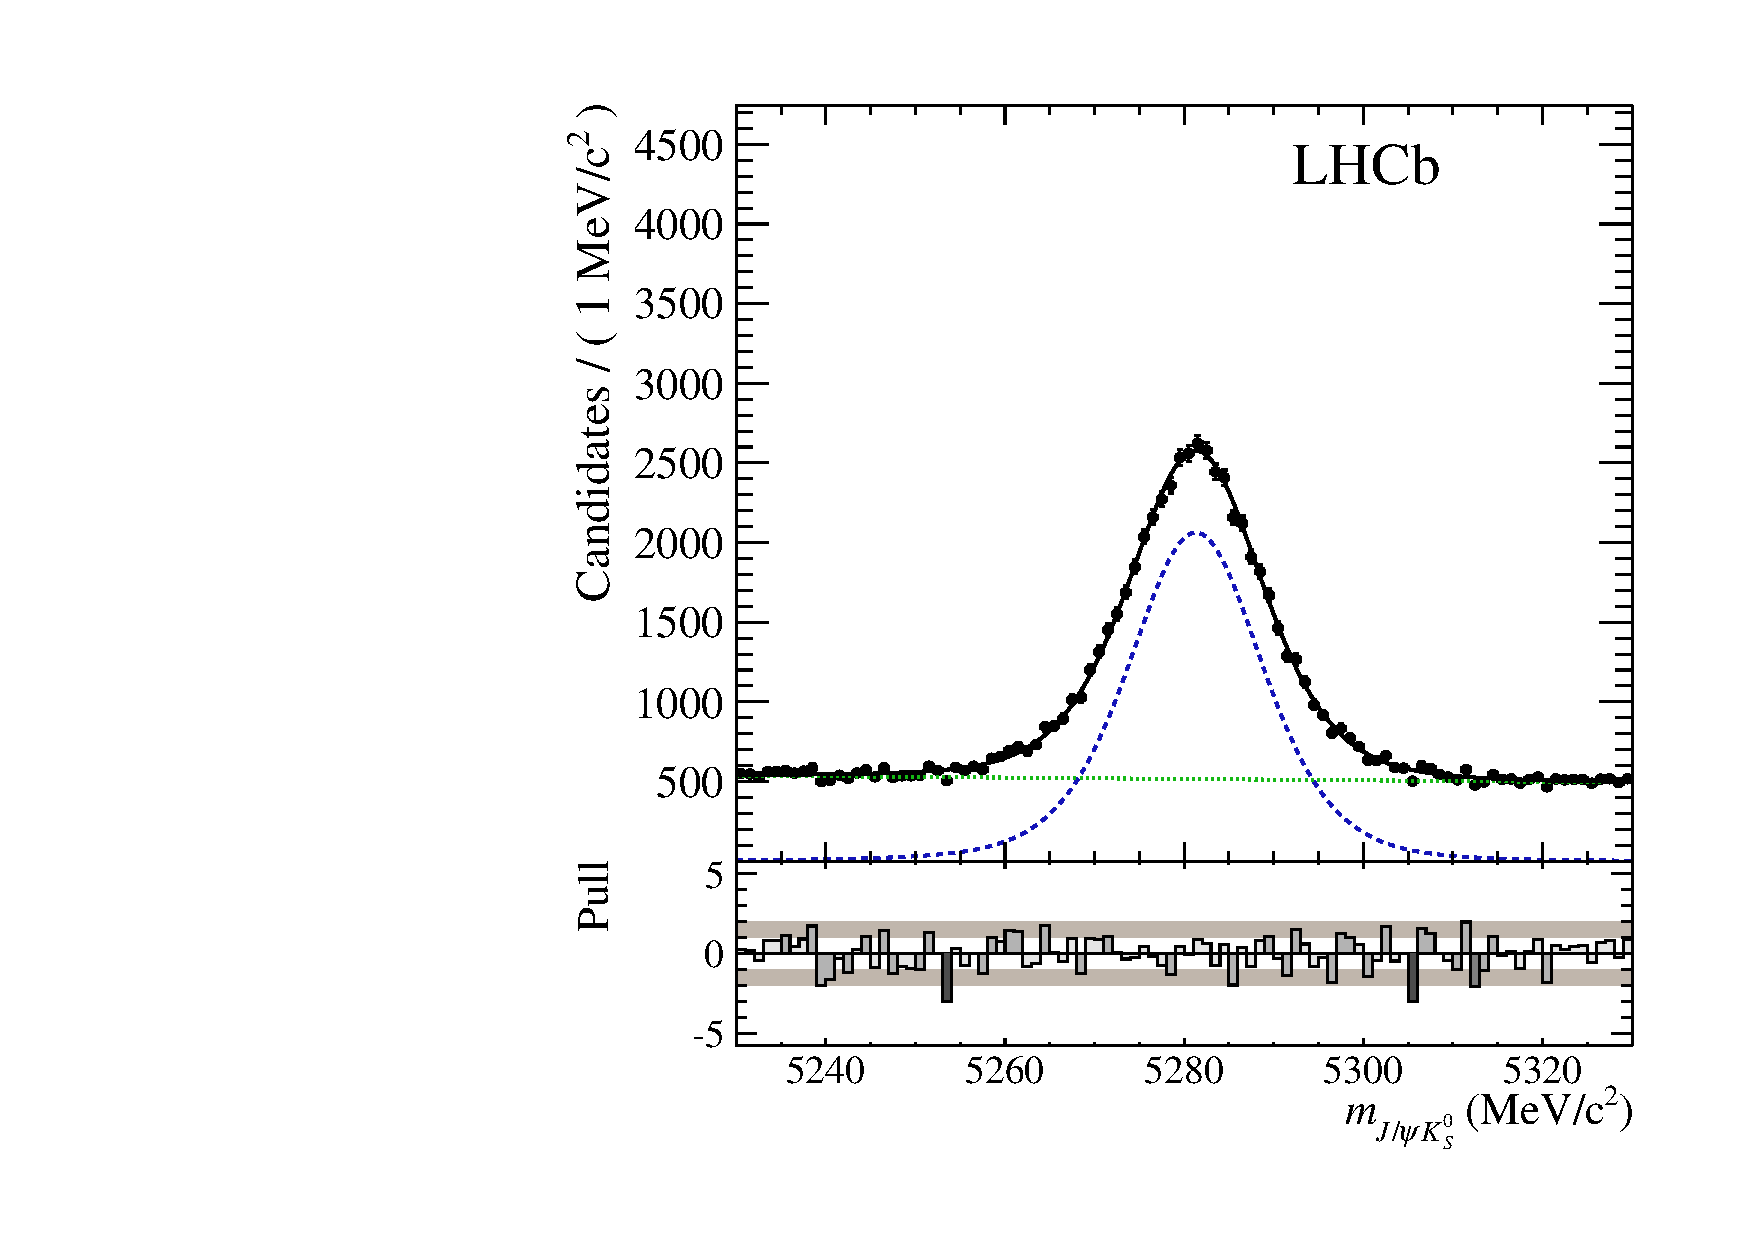
\includegraphics[width=0.49\textwidth]{private/content/measurement-of-sin2beta/figs/obsMass_summed_pull.pdf} 
  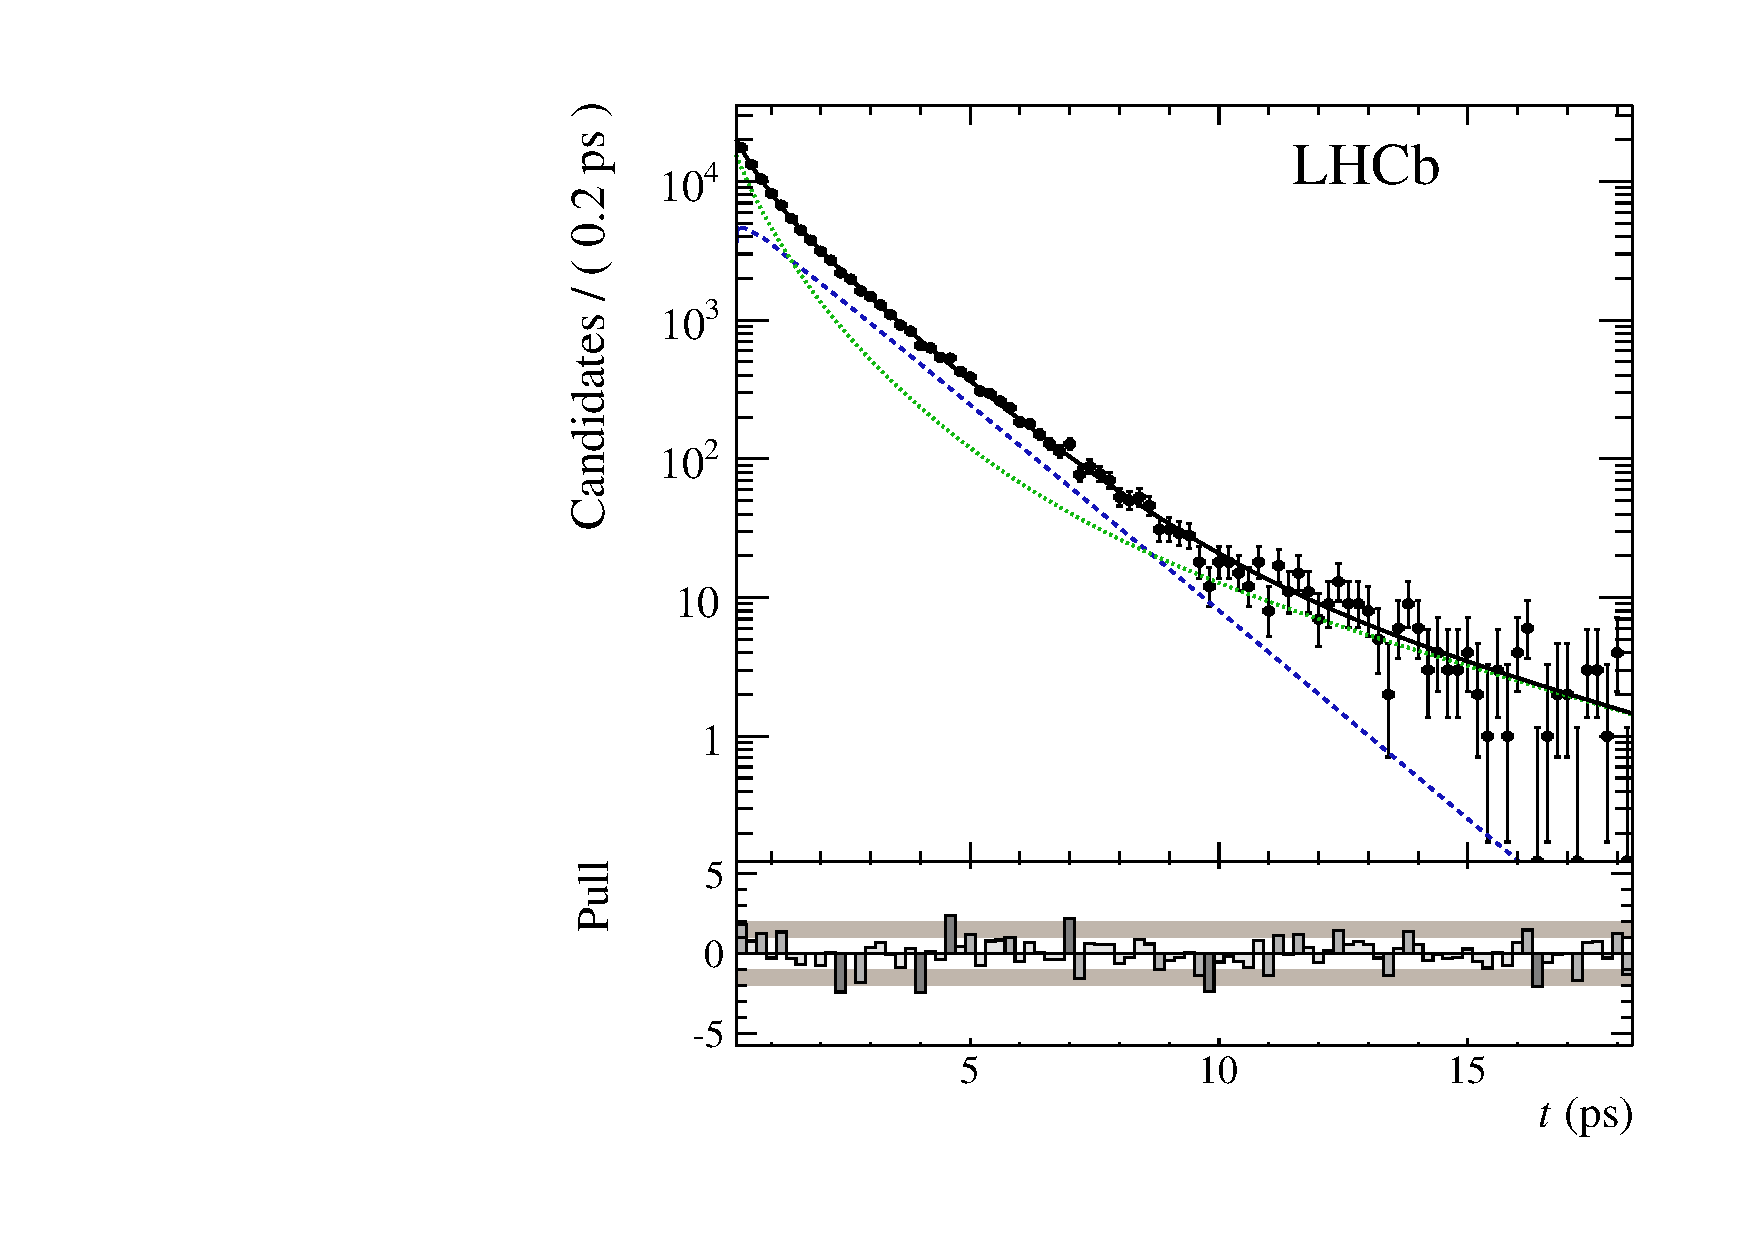
\includegraphics[width=0.49\textwidth]{private/content/measurement-of-sin2beta/figs/obsTime_summed_pull_log.pdf} \\
  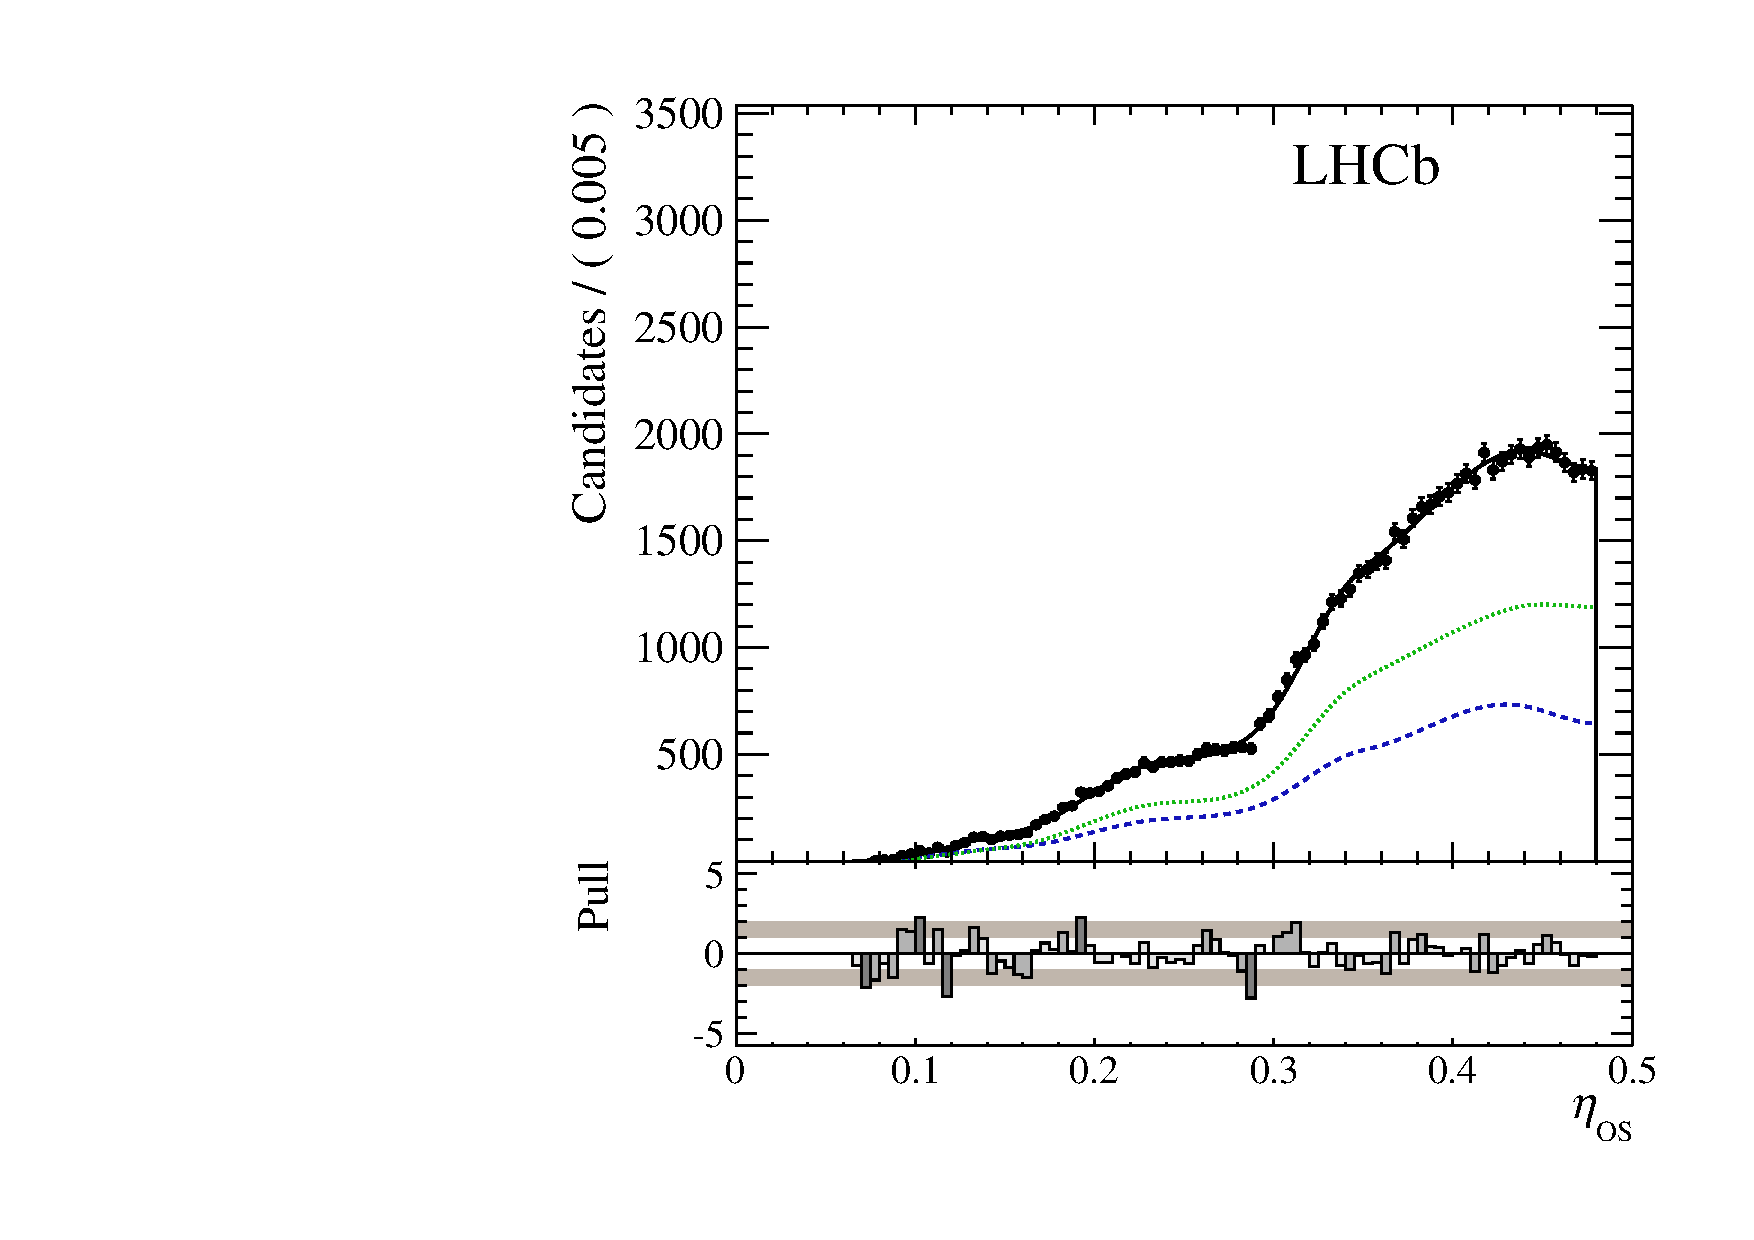
\includegraphics[width=0.315\textwidth]{private/content/measurement-of-sin2beta/figs/obsEtaOS_StdComb_CutOff_summed_pull.pdf}
  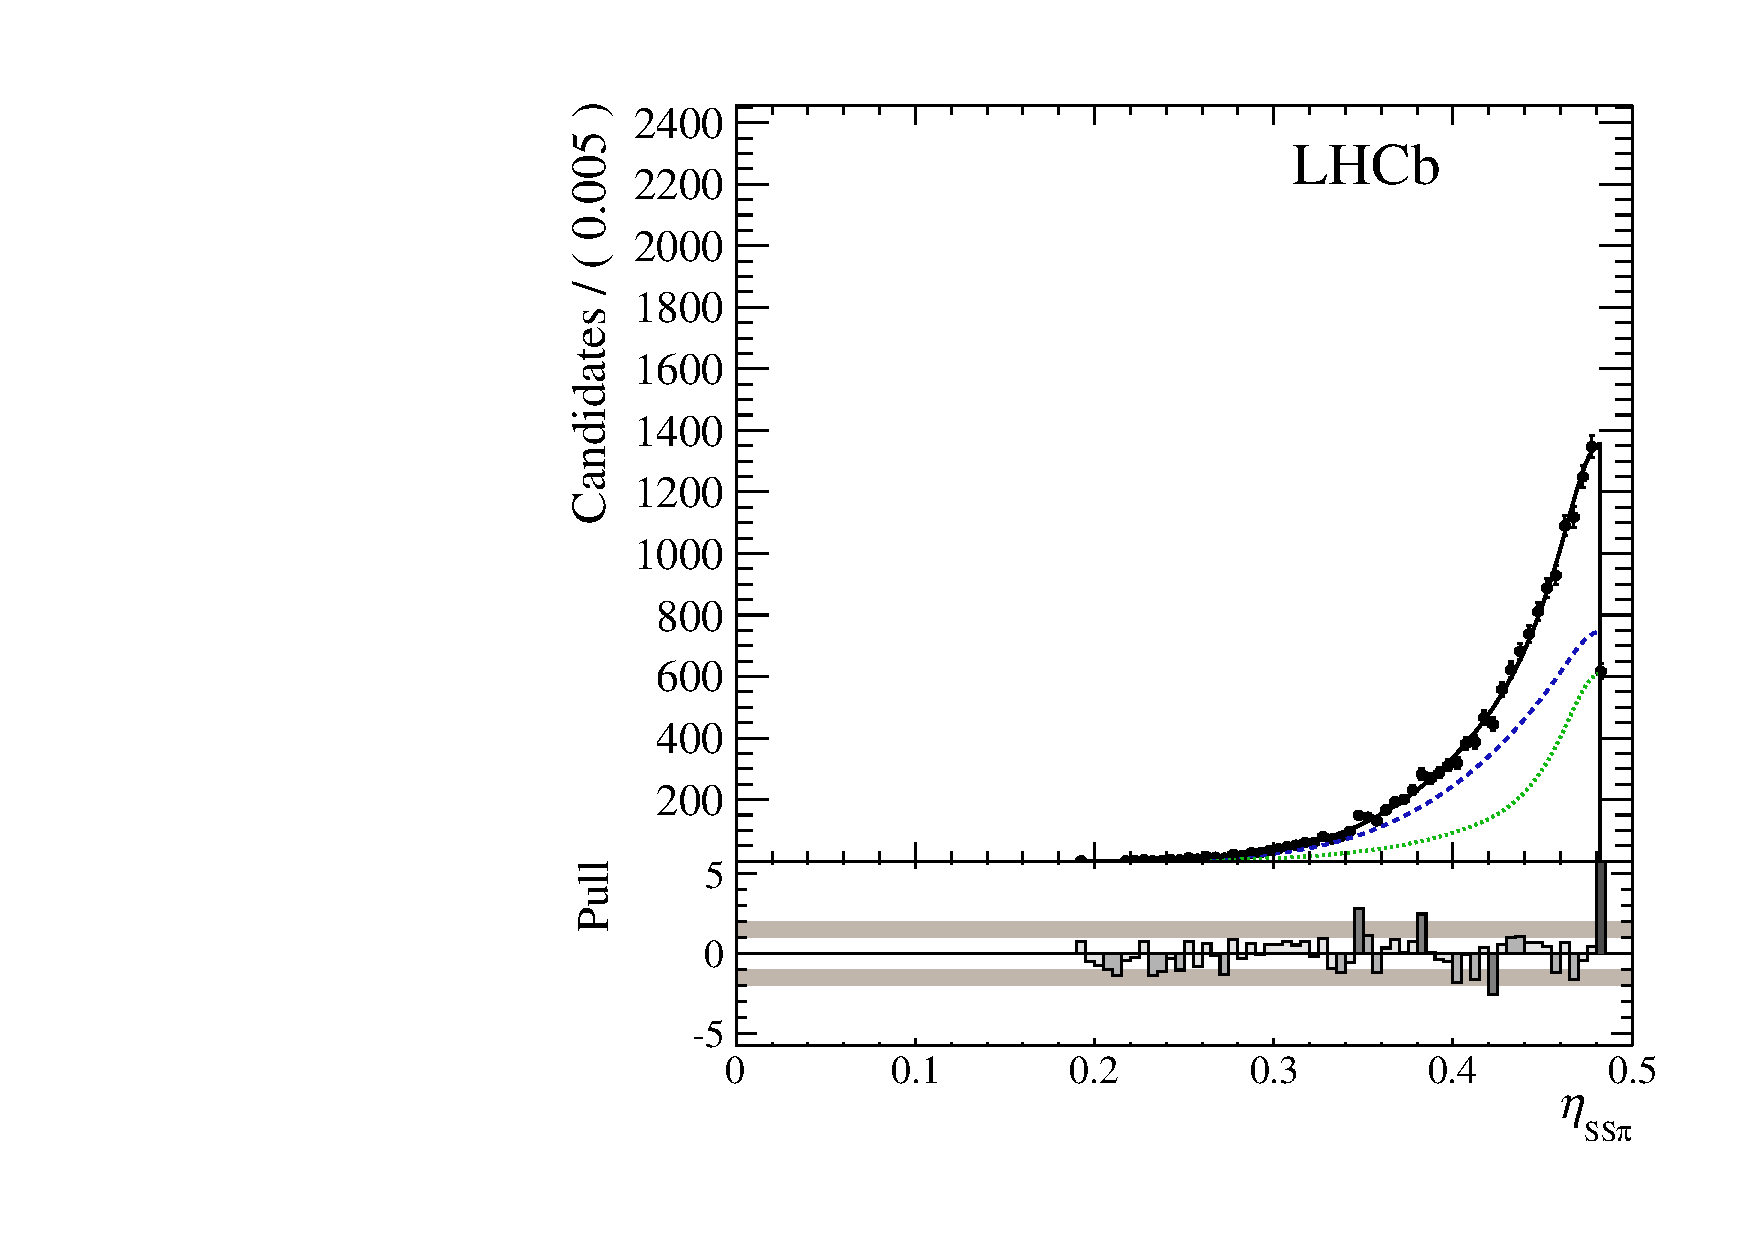
\includegraphics[width=0.315\textwidth]{private/content/measurement-of-sin2beta/figs/obsEtaSSPion_TupleCalib_summed_pull.pdf}
  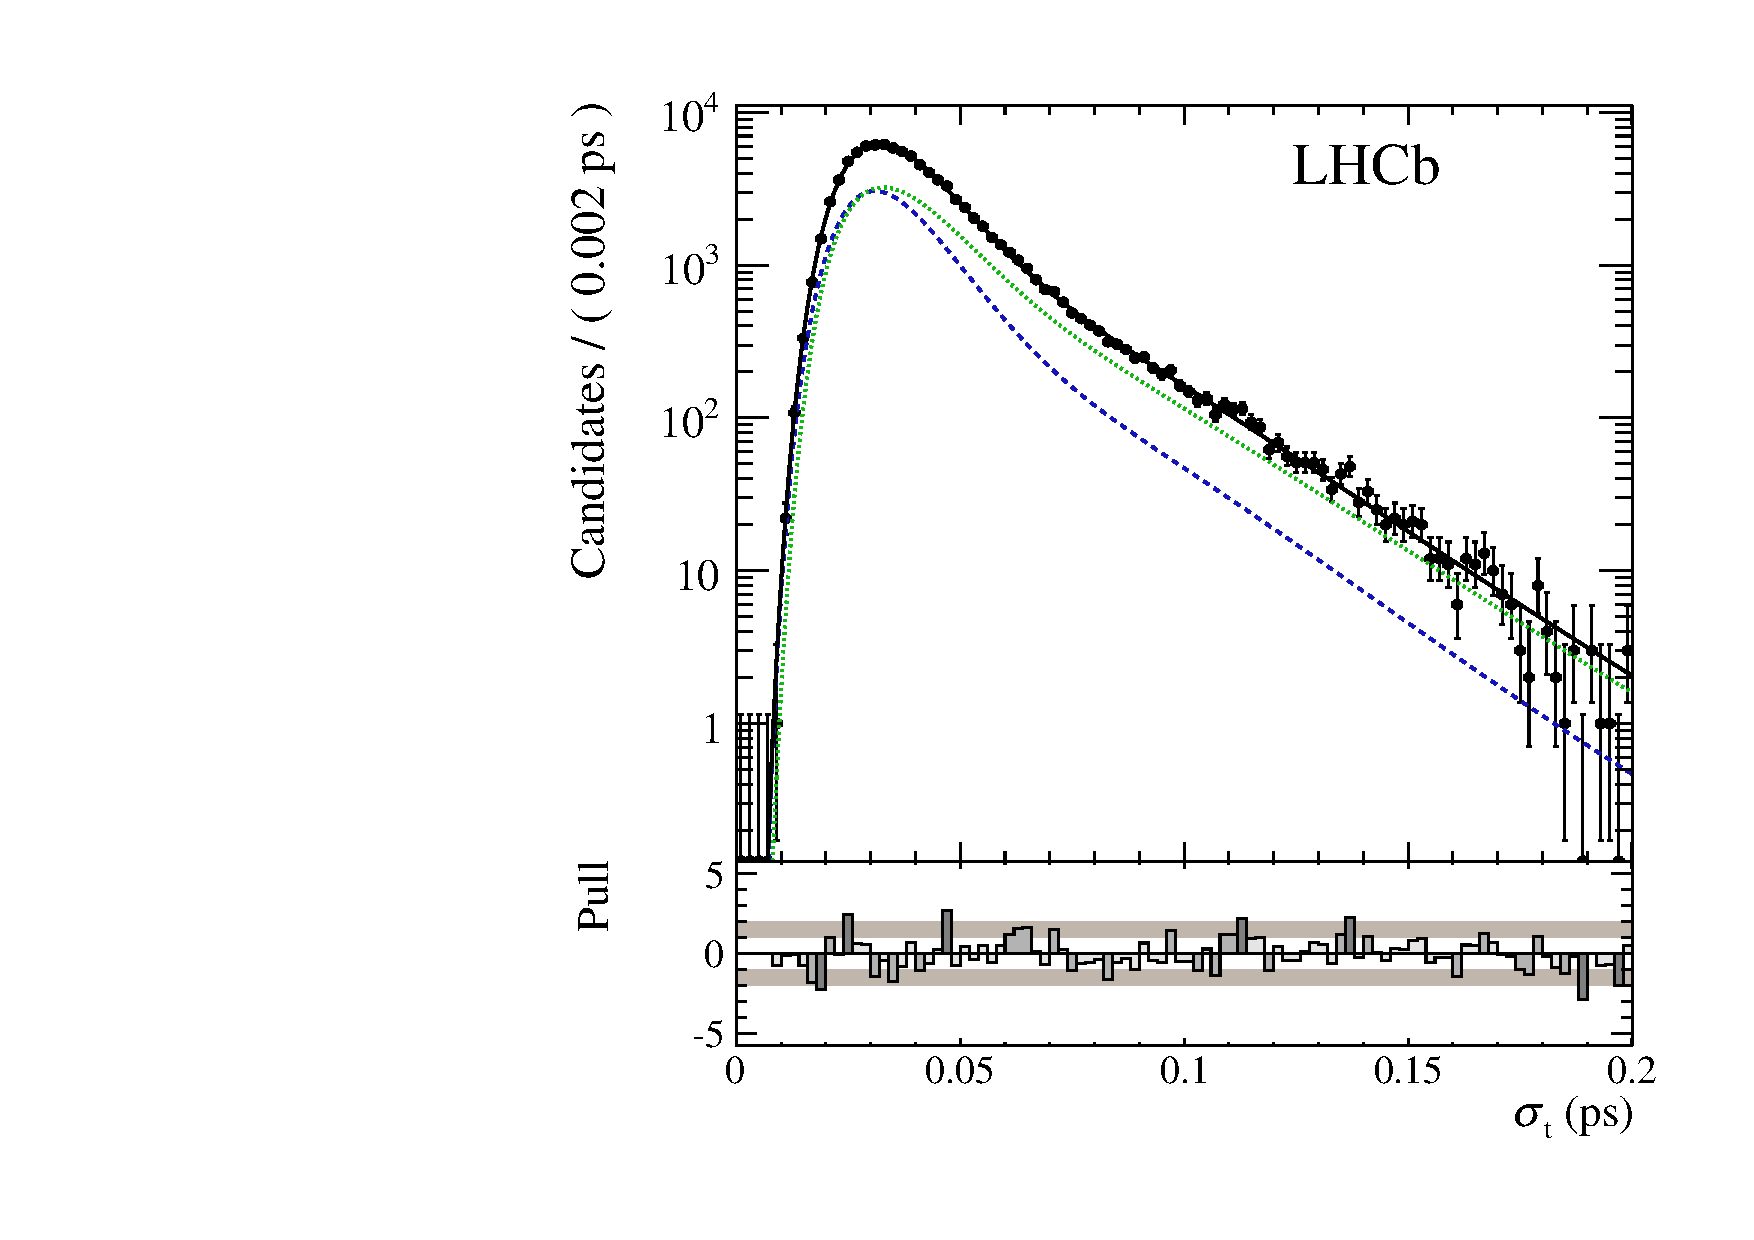
\includegraphics[width=0.315\textwidth]{private/content/measurement-of-sin2beta/figs/obsTimeError_summed_pull_log.pdf}
  \caption{Plots of the \BdToJpsiKS data sample with the projected \ac{PDF} and
  pull distributions. Shown is the reconstructed mass \obsMass (top left) and
  decay time \obsTime (top right, logarithmic), per-event mistag (bottom left
  \obsEtaOS, bottom center \obsEtaSS), and decay time error \obsTimeError (bottom
  right, logarithmic). Besides the data points and the full
  \ac{PDF} (solid black) the projections of the signal (dashed blue) and the
  background (dotted green) are shown.}
  \label{fig:measurement_of_sin2beta:cpv_measurement:results:plots:dimensions}
\end{figure}
%
\begin{figure}
\centering
  \begin{tikzpicture}[scale=0.7]
  %!TEX root = ../main.tex
%\begin{tikzpicture}
\pgfdeclareplotmark{cross} {
\pgfpathmoveto{\pgfpoint{-0.3\pgfplotmarksize}{\pgfplotmarksize}}
\pgfpathlineto{\pgfpoint{+0.3\pgfplotmarksize}{\pgfplotmarksize}}
\pgfpathlineto{\pgfpoint{+0.3\pgfplotmarksize}{0.3\pgfplotmarksize}}
\pgfpathlineto{\pgfpoint{+1\pgfplotmarksize}{0.3\pgfplotmarksize}}
\pgfpathlineto{\pgfpoint{+1\pgfplotmarksize}{-0.3\pgfplotmarksize}}
\pgfpathlineto{\pgfpoint{+0.3\pgfplotmarksize}{-0.3\pgfplotmarksize}}
\pgfpathlineto{\pgfpoint{+0.3\pgfplotmarksize}{-1.\pgfplotmarksize}}
\pgfpathlineto{\pgfpoint{-0.3\pgfplotmarksize}{-1.\pgfplotmarksize}}
\pgfpathlineto{\pgfpoint{-0.3\pgfplotmarksize}{-0.3\pgfplotmarksize}}
\pgfpathlineto{\pgfpoint{-1.\pgfplotmarksize}{-0.3\pgfplotmarksize}}
\pgfpathlineto{\pgfpoint{-1.\pgfplotmarksize}{0.3\pgfplotmarksize}}
\pgfpathlineto{\pgfpoint{-0.3\pgfplotmarksize}{0.3\pgfplotmarksize}}
\pgfpathclose
\pgfusepathqstroke
}
\pgfdeclareplotmark{cross*} {
\pgfpathmoveto{\pgfpoint{-0.3\pgfplotmarksize}{\pgfplotmarksize}}
\pgfpathlineto{\pgfpoint{+0.3\pgfplotmarksize}{\pgfplotmarksize}}
\pgfpathlineto{\pgfpoint{+0.3\pgfplotmarksize}{0.3\pgfplotmarksize}}
\pgfpathlineto{\pgfpoint{+1\pgfplotmarksize}{0.3\pgfplotmarksize}}
\pgfpathlineto{\pgfpoint{+1\pgfplotmarksize}{-0.3\pgfplotmarksize}}
\pgfpathlineto{\pgfpoint{+0.3\pgfplotmarksize}{-0.3\pgfplotmarksize}}
\pgfpathlineto{\pgfpoint{+0.3\pgfplotmarksize}{-1.\pgfplotmarksize}}
\pgfpathlineto{\pgfpoint{-0.3\pgfplotmarksize}{-1.\pgfplotmarksize}}
\pgfpathlineto{\pgfpoint{-0.3\pgfplotmarksize}{-0.3\pgfplotmarksize}}
\pgfpathlineto{\pgfpoint{-1.\pgfplotmarksize}{-0.3\pgfplotmarksize}}
\pgfpathlineto{\pgfpoint{-1.\pgfplotmarksize}{0.3\pgfplotmarksize}}
\pgfpathlineto{\pgfpoint{-0.3\pgfplotmarksize}{0.3\pgfplotmarksize}}
\pgfpathclose
\pgfusepathqfillstroke
}
\pgfdeclareplotmark{newstar} {
\pgfpathmoveto{\pgfqpoint{0pt}{\pgfplotmarksize}}
\pgfpathlineto{\pgfqpointpolar{44}{0.5\pgfplotmarksize}}
\pgfpathlineto{\pgfqpointpolar{18}{\pgfplotmarksize}}
\pgfpathlineto{\pgfqpointpolar{-20}{0.5\pgfplotmarksize}}
\pgfpathlineto{\pgfqpointpolar{-54}{\pgfplotmarksize}}
\pgfpathlineto{\pgfqpointpolar{-90}{0.5\pgfplotmarksize}}
\pgfpathlineto{\pgfqpointpolar{234}{\pgfplotmarksize}}
\pgfpathlineto{\pgfqpointpolar{198}{0.5\pgfplotmarksize}}
\pgfpathlineto{\pgfqpointpolar{162}{\pgfplotmarksize}}
\pgfpathlineto{\pgfqpointpolar{134}{0.5\pgfplotmarksize}}
\pgfpathclose
\pgfusepathqstroke
}
\pgfdeclareplotmark{newstar*} {
\pgfpathmoveto{\pgfqpoint{0pt}{\pgfplotmarksize}}
\pgfpathlineto{\pgfqpointpolar{44}{0.5\pgfplotmarksize}}
\pgfpathlineto{\pgfqpointpolar{18}{\pgfplotmarksize}}
\pgfpathlineto{\pgfqpointpolar{-20}{0.5\pgfplotmarksize}}
\pgfpathlineto{\pgfqpointpolar{-54}{\pgfplotmarksize}}
\pgfpathlineto{\pgfqpointpolar{-90}{0.5\pgfplotmarksize}}
\pgfpathlineto{\pgfqpointpolar{234}{\pgfplotmarksize}}
\pgfpathlineto{\pgfqpointpolar{198}{0.5\pgfplotmarksize}}
\pgfpathlineto{\pgfqpointpolar{162}{\pgfplotmarksize}}
\pgfpathlineto{\pgfqpointpolar{134}{0.5\pgfplotmarksize}}
\pgfpathclose
\pgfusepathqfillstroke
}

\definecolor{csig}{RGB}{24,90,169}

\definecolor{c}{rgb}{1,1,1};
\draw [color=c, fill=c] (0.4,0) rectangle (19.6,13.1687);
\draw [color=c, fill=c] (3.472,2.107) rectangle (18.64,12.5103);
\definecolor{c}{rgb}{0,0,0};
\draw [c] (3.472,2.107) -- (3.472,12.5103) -- (18.64,12.5103) -- (18.64,2.107) -- (3.472,2.107);
\definecolor{c}{rgb}{1,1,1};
\draw [color=c, fill=c] (3.472,2.107) rectangle (18.64,12.5103);
\definecolor{c}{rgb}{0,0,0};
\draw [c] (3.472,2.107) -- (3.472,12.5103) -- (18.64,12.5103) -- (18.64,2.107) -- (3.472,2.107);
\draw [c] (3.472,2.107) -- (18.64,2.107);
\draw [anchor= east] (18.64,0.2) node[scale=0.9, rotate=0]{$t$\,$\mathrm{(ps)}$};
\draw [c] (7.43253,2.4191) -- (7.43253,2.107);
\draw [c] (8.2752,2.26305) -- (8.2752,2.107);
\draw [c] (9.11787,2.26305) -- (9.11787,2.107);
\draw [c] (9.96053,2.26305) -- (9.96053,2.107);
\draw [c] (10.8032,2.26305) -- (10.8032,2.107);
\draw [c] (11.6459,2.4191) -- (11.6459,2.107);
\draw [c] (12.4885,2.26305) -- (12.4885,2.107);
\draw [c] (13.3312,2.26305) -- (13.3312,2.107);
\draw [c] (14.1739,2.26305) -- (14.1739,2.107);
\draw [c] (15.0165,2.26305) -- (15.0165,2.107);
\draw [c] (15.8592,2.4191) -- (15.8592,2.107);
\draw [c] (7.43253,2.4191) -- (7.43253,2.107);
\draw [c] (6.58987,2.26305) -- (6.58987,2.107);
\draw [c] (5.7472,2.26305) -- (5.7472,2.107);
\draw [c] (4.90453,2.26305) -- (4.90453,2.107);
\draw [c] (4.06187,2.26305) -- (4.06187,2.107);
\draw [c] (15.8592,2.4191) -- (15.8592,2.107);
\draw [c] (16.7019,2.26305) -- (16.7019,2.107);
\draw [c] (17.5445,2.26305) -- (17.5445,2.107);
\draw [c] (18.3872,2.26305) -- (18.3872,2.107);
\draw [anchor=base] (7.43253,1.1) node[scale=0.9, rotate=0]{$5$};
\draw [anchor=base] (11.6459,1.1) node[scale=0.9, rotate=0]{$10$};
\draw [anchor=base] (15.8592,1.1) node[scale=0.9, rotate=0]{$15$};
\draw [c] (3.472,12.5103) -- (18.64,12.5103);
\draw [c] (7.43253,12.1982) -- (7.43253,12.5103);
\draw [c] (8.2752,12.3543) -- (8.2752,12.5103);
\draw [c] (9.11787,12.3543) -- (9.11787,12.5103);
\draw [c] (9.96053,12.3543) -- (9.96053,12.5103);
\draw [c] (10.8032,12.3543) -- (10.8032,12.5103);
\draw [c] (11.6459,12.1982) -- (11.6459,12.5103);
\draw [c] (12.4885,12.3543) -- (12.4885,12.5103);
\draw [c] (13.3312,12.3543) -- (13.3312,12.5103);
\draw [c] (14.1739,12.3543) -- (14.1739,12.5103);
\draw [c] (15.0165,12.3543) -- (15.0165,12.5103);
\draw [c] (15.8592,12.1982) -- (15.8592,12.5103);
\draw [c] (7.43253,12.1982) -- (7.43253,12.5103);
\draw [c] (6.58987,12.3543) -- (6.58987,12.5103);
\draw [c] (5.7472,12.3543) -- (5.7472,12.5103);
\draw [c] (4.90453,12.3543) -- (4.90453,12.5103);
\draw [c] (4.06187,12.3543) -- (4.06187,12.5103);
\draw [c] (15.8592,12.1982) -- (15.8592,12.5103);
\draw [c] (16.7019,12.3543) -- (16.7019,12.5103);
\draw [c] (17.5445,12.3543) -- (17.5445,12.5103);
\draw [c] (18.3872,12.3543) -- (18.3872,12.5103);
\draw [c] (3.472,2.107) -- (3.472,12.5103);
\draw [anchor= east] (0.,12.5103) node[scale=0.9, rotate=90]{Signal-yield asymmetry};
\draw [c] (3.92704,2.107) -- (3.472,2.107);
\draw [c] (3.69952,2.36708) -- (3.472,2.36708);
\draw [c] (3.69952,2.62717) -- (3.472,2.62717);
\draw [c] (3.69952,2.88725) -- (3.472,2.88725);
\draw [c] (3.69952,3.14733) -- (3.472,3.14733);
\draw [c] (3.92704,3.40741) -- (3.472,3.40741);
\draw [c] (3.69952,3.6675) -- (3.472,3.6675);
\draw [c] (3.69952,3.92758) -- (3.472,3.92758);
\draw [c] (3.69952,4.18766) -- (3.472,4.18766);
\draw [c] (3.69952,4.44775) -- (3.472,4.44775);
\draw [c] (3.92704,4.70783) -- (3.472,4.70783);
\draw [c] (3.69952,4.96791) -- (3.472,4.96791);
\draw [c] (3.69952,5.22799) -- (3.472,5.22799);
\draw [c] (3.69952,5.48808) -- (3.472,5.48808);
\draw [c] (3.69952,5.74816) -- (3.472,5.74816);
\draw [c] (3.92704,6.00824) -- (3.472,6.00824);
\draw [c] (3.69952,6.26832) -- (3.472,6.26832);
\draw [c] (3.69952,6.52841) -- (3.472,6.52841);
\draw [c] (3.69952,6.78849) -- (3.472,6.78849);
\draw [c] (3.69952,7.04857) -- (3.472,7.04857);
\draw [c] (3.92704,7.30866) -- (3.472,7.30866);
\draw [c] (3.69952,7.56874) -- (3.472,7.56874);
\draw [c] (3.69952,7.82882) -- (3.472,7.82882);
\draw [c] (3.69952,8.0889) -- (3.472,8.0889);
\draw [c] (3.69952,8.34899) -- (3.472,8.34899);
\draw [c] (3.92704,8.60907) -- (3.472,8.60907);
\draw [c] (3.69952,8.86915) -- (3.472,8.86915);
\draw [c] (3.69952,9.12924) -- (3.472,9.12924);
\draw [c] (3.69952,9.38932) -- (3.472,9.38932);
\draw [c] (3.69952,9.6494) -- (3.472,9.6494);
\draw [c] (3.92704,9.90948) -- (3.472,9.90948);
\draw [c] (3.69952,10.1696) -- (3.472,10.1696);
\draw [c] (3.69952,10.4297) -- (3.472,10.4297);
\draw [c] (3.69952,10.6897) -- (3.472,10.6897);
\draw [c] (3.69952,10.9498) -- (3.472,10.9498);
\draw [c] (3.92704,11.2099) -- (3.472,11.2099);
\draw [c] (3.69952,11.47) -- (3.472,11.47);
\draw [c] (3.69952,11.7301) -- (3.472,11.7301);
\draw [c] (3.69952,11.9901) -- (3.472,11.9901);
\draw [c] (3.69952,12.2502) -- (3.472,12.2502);
\draw [c] (3.92704,12.5103) -- (3.472,12.5103);
\draw [anchor= east] (3.5,2.107)   node[scale=0.9, rotate=0]{$-0.4$};
\draw [anchor= east] (3.5,3.40741) node[scale=0.9, rotate=0]{$-0.3$};
\draw [anchor= east] (3.5,4.70783) node[scale=0.9, rotate=0]{$-0.2$};
\draw [anchor= east] (3.5,6.00824) node[scale=0.9, rotate=0]{$-0.1$};
\draw [anchor= east] (3.5,7.30866) node[scale=0.9, rotate=0]{$0$};
\draw [anchor= east] (3.5,8.60907) node[scale=0.9, rotate=0]{$0.1$};
\draw [anchor= east] (3.5,9.90948) node[scale=0.9, rotate=0]{$0.2$};
\draw [anchor= east] (3.5,11.2099) node[scale=0.9, rotate=0]{$0.3$};
\draw [anchor= east] (3.5,12.5103) node[scale=0.9, rotate=0]{$0.4$};
\draw [c] (18.64,2.107) -- (18.64,12.5103);
\draw [c] (18.185,2.107) -- (18.64,2.107);
\draw [c] (18.4125,2.36708) -- (18.64,2.36708);
\draw [c] (18.4125,2.62717) -- (18.64,2.62717);
\draw [c] (18.4125,2.88725) -- (18.64,2.88725);
\draw [c] (18.4125,3.14733) -- (18.64,3.14733);
\draw [c] (18.185,3.40741) -- (18.64,3.40741);
\draw [c] (18.4125,3.6675) -- (18.64,3.6675);
\draw [c] (18.4125,3.92758) -- (18.64,3.92758);
\draw [c] (18.4125,4.18766) -- (18.64,4.18766);
\draw [c] (18.4125,4.44775) -- (18.64,4.44775);
\draw [c] (18.185,4.70783) -- (18.64,4.70783);
\draw [c] (18.4125,4.96791) -- (18.64,4.96791);
\draw [c] (18.4125,5.22799) -- (18.64,5.22799);
\draw [c] (18.4125,5.48808) -- (18.64,5.48808);
\draw [c] (18.4125,5.74816) -- (18.64,5.74816);
\draw [c] (18.185,6.00824) -- (18.64,6.00824);
\draw [c] (18.4125,6.26832) -- (18.64,6.26832);
\draw [c] (18.4125,6.52841) -- (18.64,6.52841);
\draw [c] (18.4125,6.78849) -- (18.64,6.78849);
\draw [c] (18.4125,7.04857) -- (18.64,7.04857);
\draw [c] (18.185,7.30866) -- (18.64,7.30866);
\draw [c] (18.4125,7.56874) -- (18.64,7.56874);
\draw [c] (18.4125,7.82882) -- (18.64,7.82882);
\draw [c] (18.4125,8.0889) -- (18.64,8.0889);
\draw [c] (18.4125,8.34899) -- (18.64,8.34899);
\draw [c] (18.185,8.60907) -- (18.64,8.60907);
\draw [c] (18.4125,8.86915) -- (18.64,8.86915);
\draw [c] (18.4125,9.12924) -- (18.64,9.12924);
\draw [c] (18.4125,9.38932) -- (18.64,9.38932);
\draw [c] (18.4125,9.6494) -- (18.64,9.6494);
\draw [c] (18.185,9.90948) -- (18.64,9.90948);
\draw [c] (18.4125,10.1696) -- (18.64,10.1696);
\draw [c] (18.4125,10.4297) -- (18.64,10.4297);
\draw [c] (18.4125,10.6897) -- (18.64,10.6897);
\draw [c] (18.4125,10.9498) -- (18.64,10.9498);
\draw [c] (18.185,11.2099) -- (18.64,11.2099);
\draw [c] (18.4125,11.47) -- (18.64,11.47);
\draw [c] (18.4125,11.7301) -- (18.64,11.7301);
\draw [c] (18.4125,11.9901) -- (18.64,11.9901);
\draw [c] (18.4125,12.2502) -- (18.64,12.2502);
\draw [c] (18.185,12.5103) -- (18.64,12.5103);
\draw [c] (3.55627,7.72485) -- (3.472,7.72485);
\draw [c] (3.472,7.68021) -- (3.472,7.7695);
\draw [c] (3.55627,7.72485) -- (3.64053,7.72485);
\draw [c] (3.64053,7.68021) -- (3.64053,7.7695);
\draw [c] (3.55627,7.72485) -- (3.55627,8.0317);
\draw [c] (3.51162,8.0317) -- (3.60091,8.0317);
\draw [c] (3.55627,7.72485) -- (3.55627,7.41801);
\draw [c] (3.51162,7.41801) -- (3.60091,7.41801);
\draw [c] (3.76693,7.99845) -- (3.64053,7.99845);
\draw [c] (3.64053,7.9538) -- (3.64053,8.04309);
\draw [c] (3.76693,7.99845) -- (3.89333,7.99845);
\draw [c] (3.89333,7.9538) -- (3.89333,8.04309);
\draw [c] (3.76693,7.99845) -- (3.76693,8.23983);
\draw [c] (3.72229,8.23983) -- (3.81158,8.23983);
\draw [c] (3.76693,7.99845) -- (3.76693,7.75706);
\draw [c] (3.72229,7.75706) -- (3.81158,7.75706);
\draw [c] (4.06187,8.48292) -- (3.89333,8.48292);
\draw [c] (3.89333,8.43828) -- (3.89333,8.52756);
\draw [c] (4.06187,8.48292) -- (4.2304,8.48292);
\draw [c] (4.2304,8.43828) -- (4.2304,8.52756);
\draw [c] (4.06187,8.48292) -- (4.06187,8.69191);
\draw [c] (4.01722,8.69191) -- (4.10651,8.69191);
\draw [c] (4.06187,8.48292) -- (4.06187,8.27393);
\draw [c] (4.01722,8.27393) -- (4.10651,8.27393);
\draw [c] (4.44107,9.13937) -- (4.2304,9.13937);
\draw [c] (4.2304,9.09473) -- (4.2304,9.18401);
\draw [c] (4.44107,9.13937) -- (4.65173,9.13937);
\draw [c] (4.65173,9.09473) -- (4.65173,9.18401);
\draw [c] (4.44107,9.13937) -- (4.44107,9.34921);
\draw [c] (4.39642,9.34921) -- (4.48571,9.34921);
\draw [c] (4.44107,9.13937) -- (4.44107,8.92953);
\draw [c] (4.39642,8.92953) -- (4.48571,8.92953);
\draw [c] (4.90453,8.99129) -- (4.65173,8.99129);
\draw [c] (4.65173,8.94665) -- (4.65173,9.03594);
\draw [c] (4.90453,8.99129) -- (5.15733,8.99129);
\draw [c] (5.15733,8.94665) -- (5.15733,9.03594);
\draw [c] (4.90453,8.99129) -- (4.90453,9.20979);
\draw [c] (4.85989,9.20979) -- (4.94918,9.20979);
\draw [c] (4.90453,8.99129) -- (4.90453,8.7728);
\draw [c] (4.85989,8.7728) -- (4.94918,8.7728);
\draw [c] (5.45227,9.53821) -- (5.15733,9.53821);
\draw [c] (5.15733,9.49356) -- (5.15733,9.58285);
\draw [c] (5.45227,9.53821) -- (5.7472,9.53821);
\draw [c] (5.7472,9.49356) -- (5.7472,9.58285);
\draw [c] (5.45227,9.53821) -- (5.45227,9.78334);
\draw [c] (5.40762,9.78334) -- (5.49691,9.78334);
\draw [c] (5.45227,9.53821) -- (5.45227,9.29307);
\draw [c] (5.40762,9.29307) -- (5.49691,9.29307);
\draw [c] (6.08427,9.73341) -- (5.7472,9.73341);
\draw [c] (5.7472,9.68876) -- (5.7472,9.77805);
\draw [c] (6.08427,9.73341) -- (6.42133,9.73341);
\draw [c] (6.42133,9.68876) -- (6.42133,9.77805);
\draw [c] (6.08427,9.73341) -- (6.08427,10.0244);
\draw [c] (6.03962,10.0244) -- (6.12891,10.0244);
\draw [c] (6.08427,9.73341) -- (6.08427,9.44242);
\draw [c] (6.03962,9.44242) -- (6.12891,9.44242);
\draw [c] (6.80053,9.14497) -- (6.42133,9.14497);
\draw [c] (6.42133,9.10033) -- (6.42133,9.18962);
\draw [c] (6.80053,9.14497) -- (7.17973,9.14497);
\draw [c] (7.17973,9.10033) -- (7.17973,9.18962);
\draw [c] (6.80053,9.14497) -- (6.80053,9.49261);
\draw [c] (6.75589,9.49261) -- (6.84518,9.49261);
\draw [c] (6.80053,9.14497) -- (6.80053,8.79734);
\draw [c] (6.75589,8.79734) -- (6.84518,8.79734);
\draw [c] (7.60107,7.8052) -- (7.17973,7.8052);
\draw [c] (7.17973,7.76056) -- (7.17973,7.84985);
\draw [c] (7.60107,7.8052) -- (8.0224,7.8052);
\draw [c] (8.0224,7.76056) -- (8.0224,7.84985);
\draw [c] (7.60107,7.8052) -- (7.60107,8.25309);
\draw [c] (7.55642,8.25309) -- (7.64571,8.25309);
\draw [c] (7.60107,7.8052) -- (7.60107,7.35732);
\draw [c] (7.55642,7.35732) -- (7.64571,7.35732);
\draw [c] (8.48587,6.91766) -- (8.0224,6.91766);
\draw [c] (8.0224,6.87302) -- (8.0224,6.96231);
\draw [c] (8.48587,6.91766) -- (8.94933,6.91766);
\draw [c] (8.94933,6.87302) -- (8.94933,6.96231);
\draw [c] (8.48587,6.91766) -- (8.48587,7.55158);
\draw [c] (8.44122,7.55158) -- (8.53051,7.55158);
\draw [c] (8.48587,6.91766) -- (8.48587,6.28375);
\draw [c] (8.44122,6.28375) -- (8.53051,6.28375);
\draw [c] (9.45493,6.43803) -- (8.94933,6.43803);
\draw [c] (8.94933,6.39339) -- (8.94933,6.48268);
\draw [c] (9.45493,6.43803) -- (9.96053,6.43803);
\draw [c] (9.96053,6.39339) -- (9.96053,6.48268);
\draw [c] (9.45493,6.43803) -- (9.45493,7.29226);
\draw [c] (9.41029,7.29226) -- (9.49958,7.29226);
\draw [c] (9.45493,6.43803) -- (9.45493,5.58381);
\draw [c] (9.41029,5.58381) -- (9.49958,5.58381);
\draw [c] (10.8032,5.85731) -- (9.96053,5.85731);
\draw [c] (9.96053,5.81267) -- (9.96053,5.90196);
\draw [c] (10.8032,5.85731) -- (11.6459,5.85731);
\draw [c] (11.6459,5.81267) -- (11.6459,5.90196);
\draw [c] (10.8032,5.85731) -- (10.8032,7.08927);
\draw [c] (10.7586,7.08927) -- (10.8478,7.08927);
\draw [c] (10.8032,5.85731) -- (10.8032,4.62536);
\draw [c] (10.7586,4.62536) -- (10.8478,4.62536);
\draw [c] (12.9099,6.6293) -- (11.6459,6.6293);
\draw [c] (11.6459,6.58465) -- (11.6459,6.67394);
\draw [c] (12.9099,6.6293) -- (14.1739,6.6293);
\draw [c] (14.1739,6.58465) -- (14.1739,6.67394);
\draw [c] (12.9099,6.6293) -- (12.9099,8.95393);
\draw [c] (12.8652,8.95393) -- (12.9545,8.95393);
\draw [c] (12.9099,6.6293) -- (12.9099,4.30466);
\draw [c] (12.8652,4.30466) -- (12.9545,4.30466);
\draw [c] (16.4069,8.21394) -- (14.1739,8.21394);
\draw [c] (14.1739,8.16929) -- (14.1739,8.25858);
\draw [c] (16.4069,8.21394) -- (18.64,8.21394);
\draw [c] (18.64,8.16929) -- (18.64,8.25858);
\draw [c] (16.4069,8.21394) -- (16.4069,12.0975);
\draw [c] (16.3623,12.0975) -- (16.4516,12.0975);
\draw [c] (16.4069,8.21394) -- (16.4069,4.33041);
\draw [c] (16.3623,4.33041) -- (16.4516,4.33041);
\foreach \P in
 {(3.55627,7.72485),(3.76693,7.99845),(4.06187,8.48292),(4.44107,9.13937),(4.90453,8.99129),(5.45227,9.53821),(6.08427,9.73341),(6.80053,9.14497),(7.60107,7.8052),(8.48587,6.91766),(9.45493,6.43803),(10.8032,5.85731),(12.9099,6.6293),(16.4069,8.21394
)}{\draw[mark options={color=c,fill=c},mark size=2.402402pt,mark=] plot coordinates {\P};}
\draw [c] (3.54784,7.30866) -- (3.69952,7.30866) -- (3.8512,7.30866) -- (4.00288,7.30866) -- (4.15456,7.30866) -- (4.30624,7.30866) -- (4.45792,7.30866) -- (4.6096,7.30866) -- (4.76128,7.30866) -- (4.91296,7.30866) -- (5.06464,7.30866) --
 (5.21632,7.30866) -- (5.368,7.30866) -- (5.51968,7.30866) -- (5.67136,7.30866) -- (5.82304,7.30866) -- (5.97472,7.30866) -- (6.1264,7.30866) -- (6.27808,7.30866) -- (6.42976,7.30866) -- (6.58144,7.30866) -- (6.73312,7.30866) -- (6.8848,7.30866) --
 (7.03648,7.30866) -- (7.18816,7.30866) -- (7.33984,7.30866) -- (7.49152,7.30866) -- (7.6432,7.30866) -- (7.79488,7.30866) -- (7.94656,7.30866) -- (8.09824,7.30866) -- (8.24992,7.30866) -- (8.4016,7.30866) -- (8.55328,7.30866) -- (8.70496,7.30866) --
 (8.85664,7.30866) -- (9.00832,7.30866) -- (9.16,7.30866) -- (9.31168,7.30866) -- (9.46336,7.30866) -- (9.61504,7.30866) -- (9.76672,7.30866) -- (9.9184,7.30866) -- (10.0701,7.30866) -- (10.2218,7.30866) -- (10.3734,7.30866) -- (10.5251,7.30866) --
 (10.6768,7.30866) -- (10.8285,7.30866) -- (10.9802,7.30866);
\draw [c] (10.9802,7.30866) -- (11.1318,7.30866) -- (11.2835,7.30866) -- (11.4352,7.30866) -- (11.5869,7.30866) -- (11.7386,7.30866) -- (11.8902,7.30866) -- (12.0419,7.30866) -- (12.1936,7.30866) -- (12.3453,7.30866) -- (12.497,7.30866) --
 (12.6486,7.30866) -- (12.8003,7.30866) -- (12.952,7.30866) -- (13.1037,7.30866) -- (13.2554,7.30866) -- (13.407,7.30866) -- (13.5587,7.30866) -- (13.7104,7.30866) -- (13.8621,7.30866) -- (14.0138,7.30866) -- (14.1654,7.30866) -- (14.3171,7.30866) --
 (14.4688,7.30866) -- (14.6205,7.30866) -- (14.7722,7.30866) -- (14.9238,7.30866) -- (15.0755,7.30866) -- (15.2272,7.30866) -- (15.3789,7.30866) -- (15.5306,7.30866) -- (15.6822,7.30866) -- (15.8339,7.30866) -- (15.9856,7.30866) -- (16.1373,7.30866)
 -- (16.289,7.30866) -- (16.4406,7.30866) -- (16.5923,7.30866) -- (16.744,7.30866) -- (16.8957,7.30866) -- (17.0474,7.30866) -- (17.199,7.30866) -- (17.3507,7.30866) -- (17.5024,7.30866) -- (17.6541,7.30866) -- (17.8058,7.30866) -- (17.9574,7.30866)
 -- (18.1091,7.30866) -- (18.2608,7.30866) -- (18.4125,7.30866);
\draw [c] (18.4125,7.30866) -- (18.5642,7.30866);
\definecolor{c}{rgb}{0.08,0.08,0.72};
\draw [csig,line width=0.6] (3.472,7.85697) -- (3.62368,8.04849) -- (3.77536,8.23217) -- (3.92704,8.40628) -- (4.07872,8.56942) -- (4.2304,8.7205) -- (4.38208,8.85867) -- (4.53376,8.98333) -- (4.68544,9.09406) -- (4.83712,9.19063) -- (4.9888,9.27292) --
 (5.14048,9.34092) -- (5.29216,9.39464) -- (5.44384,9.43413) -- (5.59552,9.45945) -- (5.7472,9.47063) -- (5.89888,9.46775) -- (6.05056,9.45082) -- (6.20224,9.41993) -- (6.35392,9.37517) -- (6.5056,9.31669) -- (6.65728,9.24471) -- (6.80896,9.15955) --
 (6.96064,9.0616) -- (7.11232,8.95142) -- (7.264,8.82963) -- (7.41568,8.69702) -- (7.56736,8.5545) -- (7.71904,8.40307) -- (7.87072,8.24387) -- (8.0224,8.07811) -- (8.17408,7.90709) -- (8.32576,7.7322) -- (8.47744,7.55484) -- (8.62912,7.37646) --
 (8.7808,7.19854) -- (8.93248,7.02254) -- (9.08416,6.84992) -- (9.23584,6.68209) -- (9.38752,6.52045) -- (9.5392,6.36632) -- (9.69088,6.22097) -- (9.84256,6.08558) -- (9.99424,5.96125) -- (10.1459,5.84899) -- (10.2976,5.74972) -- (10.4493,5.66422) --
 (10.601,5.59319) -- (10.7526,5.53721) -- (10.9043,5.49671) -- (11.056,5.47202) -- (11.2077,5.46333) -- (11.3594,5.47072) -- (11.511,5.49412) -- (11.6627,5.53336) -- (11.8144,5.58809) -- (11.9661,5.65791) -- (12.1178,5.74223) -- (12.2694,5.84038) --
 (12.4211,5.95157) -- (12.5728,6.0749) -- (12.7245,6.20937) -- (12.8762,6.35387) -- (13.0278,6.50722) -- (13.1795,6.66818) -- (13.3312,6.8354) -- (13.4829,7.00751) -- (13.6346,7.18307) -- (13.7862,7.36061) -- (13.9379,7.53864) -- (14.0896,7.71567) --
 (14.2413,7.89018) -- (14.393,8.06071) -- (14.5446,8.22577) -- (14.6963,8.38396) -- (14.848,8.53392) -- (14.9997,8.67434) -- (15.1514,8.804) -- (15.303,8.92178) -- (15.4547,9.02663) -- (15.6064,9.11765) -- (15.7581,9.19404) -- (15.9098,9.2551) --
 (16.0614,9.30032) -- (16.2131,9.32929) -- (16.3648,9.34175) -- (16.5165,9.3376) -- (16.6682,9.31687) -- (16.8198,9.27976) -- (16.9715,9.22657) -- (17.1232,9.15779) -- (17.2749,9.07405) -- (17.4266,8.97603) -- (17.5782,8.86465) -- (17.7299,8.74087)
 -- (17.8816,8.60576) -- (18.0333,8.46051) -- (18.185,8.30638) -- (18.3366,8.14469) -- (18.4883,7.97686) -- (18.64,7.8043);
\definecolor{c}{rgb}{0,0,0};
\draw [c] (3.55627,7.72485) -- (3.472,7.72485);
\draw [c] (3.472,7.68021) -- (3.472,7.7695);
\draw [c] (3.55627,7.72485) -- (3.64053,7.72485);
\draw [c] (3.64053,7.68021) -- (3.64053,7.7695);
\draw [c] (3.55627,7.72485) -- (3.55627,8.0317);
\draw [c] (3.51162,8.0317) -- (3.60091,8.0317);
\draw [c] (3.55627,7.72485) -- (3.55627,7.41801);
\draw [c] (3.51162,7.41801) -- (3.60091,7.41801);
\draw [c] (3.76693,7.99845) -- (3.64053,7.99845);
\draw [c] (3.64053,7.9538) -- (3.64053,8.04309);
\draw [c] (3.76693,7.99845) -- (3.89333,7.99845);
\draw [c] (3.89333,7.9538) -- (3.89333,8.04309);
\draw [c] (3.76693,7.99845) -- (3.76693,8.23983);
\draw [c] (3.72229,8.23983) -- (3.81158,8.23983);
\draw [c] (3.76693,7.99845) -- (3.76693,7.75706);
\draw [c] (3.72229,7.75706) -- (3.81158,7.75706);
\draw [c] (4.06187,8.48292) -- (3.89333,8.48292);
\draw [c] (3.89333,8.43828) -- (3.89333,8.52756);
\draw [c] (4.06187,8.48292) -- (4.2304,8.48292);
\draw [c] (4.2304,8.43828) -- (4.2304,8.52756);
\draw [c] (4.06187,8.48292) -- (4.06187,8.69191);
\draw [c] (4.01722,8.69191) -- (4.10651,8.69191);
\draw [c] (4.06187,8.48292) -- (4.06187,8.27393);
\draw [c] (4.01722,8.27393) -- (4.10651,8.27393);
\draw [c] (4.44107,9.13937) -- (4.2304,9.13937);
\draw [c] (4.2304,9.09473) -- (4.2304,9.18401);
\draw [c] (4.44107,9.13937) -- (4.65173,9.13937);
\draw [c] (4.65173,9.09473) -- (4.65173,9.18401);
\draw [c] (4.44107,9.13937) -- (4.44107,9.34921);
\draw [c] (4.39642,9.34921) -- (4.48571,9.34921);
\draw [c] (4.44107,9.13937) -- (4.44107,8.92953);
\draw [c] (4.39642,8.92953) -- (4.48571,8.92953);
\draw [c] (4.90453,8.99129) -- (4.65173,8.99129);
\draw [c] (4.65173,8.94665) -- (4.65173,9.03594);
\draw [c] (4.90453,8.99129) -- (5.15733,8.99129);
\draw [c] (5.15733,8.94665) -- (5.15733,9.03594);
\draw [c] (4.90453,8.99129) -- (4.90453,9.20979);
\draw [c] (4.85989,9.20979) -- (4.94918,9.20979);
\draw [c] (4.90453,8.99129) -- (4.90453,8.7728);
\draw [c] (4.85989,8.7728) -- (4.94918,8.7728);
\draw [c] (5.45227,9.53821) -- (5.15733,9.53821);
\draw [c] (5.15733,9.49356) -- (5.15733,9.58285);
\draw [c] (5.45227,9.53821) -- (5.7472,9.53821);
\draw [c] (5.7472,9.49356) -- (5.7472,9.58285);
\draw [c] (5.45227,9.53821) -- (5.45227,9.78334);
\draw [c] (5.40762,9.78334) -- (5.49691,9.78334);
\draw [c] (5.45227,9.53821) -- (5.45227,9.29307);
\draw [c] (5.40762,9.29307) -- (5.49691,9.29307);
\draw [c] (6.08427,9.73341) -- (5.7472,9.73341);
\draw [c] (5.7472,9.68876) -- (5.7472,9.77805);
\draw [c] (6.08427,9.73341) -- (6.42133,9.73341);
\draw [c] (6.42133,9.68876) -- (6.42133,9.77805);
\draw [c] (6.08427,9.73341) -- (6.08427,10.0244);
\draw [c] (6.03962,10.0244) -- (6.12891,10.0244);
\draw [c] (6.08427,9.73341) -- (6.08427,9.44242);
\draw [c] (6.03962,9.44242) -- (6.12891,9.44242);
\draw [c] (6.80053,9.14497) -- (6.42133,9.14497);
\draw [c] (6.42133,9.10033) -- (6.42133,9.18962);
\draw [c] (6.80053,9.14497) -- (7.17973,9.14497);
\draw [c] (7.17973,9.10033) -- (7.17973,9.18962);
\draw [c] (6.80053,9.14497) -- (6.80053,9.49261);
\draw [c] (6.75589,9.49261) -- (6.84518,9.49261);
\draw [c] (6.80053,9.14497) -- (6.80053,8.79734);
\draw [c] (6.75589,8.79734) -- (6.84518,8.79734);
\draw [c] (7.60107,7.8052) -- (7.17973,7.8052);
\draw [c] (7.17973,7.76056) -- (7.17973,7.84985);
\draw [c] (7.60107,7.8052) -- (8.0224,7.8052);
\draw [c] (8.0224,7.76056) -- (8.0224,7.84985);
\draw [c] (7.60107,7.8052) -- (7.60107,8.25309);
\draw [c] (7.55642,8.25309) -- (7.64571,8.25309);
\draw [c] (7.60107,7.8052) -- (7.60107,7.35732);
\draw [c] (7.55642,7.35732) -- (7.64571,7.35732);
\draw [c] (8.48587,6.91766) -- (8.0224,6.91766);
\draw [c] (8.0224,6.87302) -- (8.0224,6.96231);
\draw [c] (8.48587,6.91766) -- (8.94933,6.91766);
\draw [c] (8.94933,6.87302) -- (8.94933,6.96231);
\draw [c] (8.48587,6.91766) -- (8.48587,7.55158);
\draw [c] (8.44122,7.55158) -- (8.53051,7.55158);
\draw [c] (8.48587,6.91766) -- (8.48587,6.28375);
\draw [c] (8.44122,6.28375) -- (8.53051,6.28375);
\draw [c] (9.45493,6.43803) -- (8.94933,6.43803);
\draw [c] (8.94933,6.39339) -- (8.94933,6.48268);
\draw [c] (9.45493,6.43803) -- (9.96053,6.43803);
\draw [c] (9.96053,6.39339) -- (9.96053,6.48268);
\draw [c] (9.45493,6.43803) -- (9.45493,7.29226);
\draw [c] (9.41029,7.29226) -- (9.49958,7.29226);
\draw [c] (9.45493,6.43803) -- (9.45493,5.58381);
\draw [c] (9.41029,5.58381) -- (9.49958,5.58381);
\draw [c] (10.8032,5.85731) -- (9.96053,5.85731);
\draw [c] (9.96053,5.81267) -- (9.96053,5.90196);
\draw [c] (10.8032,5.85731) -- (11.6459,5.85731);
\draw [c] (11.6459,5.81267) -- (11.6459,5.90196);
\draw [c] (10.8032,5.85731) -- (10.8032,7.08927);
\draw [c] (10.7586,7.08927) -- (10.8478,7.08927);
\draw [c] (10.8032,5.85731) -- (10.8032,4.62536);
\draw [c] (10.7586,4.62536) -- (10.8478,4.62536);
\draw [c] (12.9099,6.6293) -- (11.6459,6.6293);
\draw [c] (11.6459,6.58465) -- (11.6459,6.67394);
\draw [c] (12.9099,6.6293) -- (14.1739,6.6293);
\draw [c] (14.1739,6.58465) -- (14.1739,6.67394);
\draw [c] (12.9099,6.6293) -- (12.9099,8.95393);
\draw [c] (12.8652,8.95393) -- (12.9545,8.95393);
\draw [c] (12.9099,6.6293) -- (12.9099,4.30466);
\draw [c] (12.8652,4.30466) -- (12.9545,4.30466);
\draw [c] (16.4069,8.21394) -- (14.1739,8.21394);
\draw [c] (14.1739,8.16929) -- (14.1739,8.25858);
\draw [c] (16.4069,8.21394) -- (18.64,8.21394);
\draw [c] (18.64,8.16929) -- (18.64,8.25858);
\draw [c] (16.4069,8.21394) -- (16.4069,12.0975);
\draw [c] (16.3623,12.0975) -- (16.4516,12.0975);
\draw [c] (16.4069,8.21394) -- (16.4069,4.33041);
\draw [c] (16.3623,4.33041) -- (16.4516,4.33041);
\foreach \P in
 {(3.55627,7.72485),(3.76693,7.99845),(4.06187,8.48292),(4.44107,9.13937),(4.90453,8.99129),(5.45227,9.53821),(6.08427,9.73341),(6.80053,9.14497),(7.60107,7.8052),(8.48587,6.91766),(9.45493,6.43803),(10.8032,5.85731),(12.9099,6.6293),(16.4069,8.21394
)}{\draw[mark options={color=c,fill=c},mark size=2.402402pt,mark=] plot coordinates {\P};}
\draw [c] (3.472,2.107) -- (18.64,2.107);
\draw [c] (7.43253,2.4191) -- (7.43253,2.107);
\draw [c] (8.2752,2.26305) -- (8.2752,2.107);
\draw [c] (9.11787,2.26305) -- (9.11787,2.107);
\draw [c] (9.96053,2.26305) -- (9.96053,2.107);
\draw [c] (10.8032,2.26305) -- (10.8032,2.107);
\draw [c] (11.6459,2.4191) -- (11.6459,2.107);
\draw [c] (12.4885,2.26305) -- (12.4885,2.107);
\draw [c] (13.3312,2.26305) -- (13.3312,2.107);
\draw [c] (14.1739,2.26305) -- (14.1739,2.107);
\draw [c] (15.0165,2.26305) -- (15.0165,2.107);
\draw [c] (15.8592,2.4191) -- (15.8592,2.107);
\draw [c] (7.43253,2.4191) -- (7.43253,2.107);
\draw [c] (6.58987,2.26305) -- (6.58987,2.107);
\draw [c] (5.7472,2.26305) -- (5.7472,2.107);
\draw [c] (4.90453,2.26305) -- (4.90453,2.107);
\draw [c] (4.06187,2.26305) -- (4.06187,2.107);
\draw [c] (15.8592,2.4191) -- (15.8592,2.107);
\draw [c] (16.7019,2.26305) -- (16.7019,2.107);
\draw [c] (17.5445,2.26305) -- (17.5445,2.107);
\draw [c] (18.3872,2.26305) -- (18.3872,2.107);
\draw [c] (3.472,12.5103) -- (18.64,12.5103);
\draw [c] (7.43253,12.1982) -- (7.43253,12.5103);
\draw [c] (8.2752,12.3543) -- (8.2752,12.5103);
\draw [c] (9.11787,12.3543) -- (9.11787,12.5103);
\draw [c] (9.96053,12.3543) -- (9.96053,12.5103);
\draw [c] (10.8032,12.3543) -- (10.8032,12.5103);
\draw [c] (11.6459,12.1982) -- (11.6459,12.5103);
\draw [c] (12.4885,12.3543) -- (12.4885,12.5103);
\draw [c] (13.3312,12.3543) -- (13.3312,12.5103);
\draw [c] (14.1739,12.3543) -- (14.1739,12.5103);
\draw [c] (15.0165,12.3543) -- (15.0165,12.5103);
\draw [c] (15.8592,12.1982) -- (15.8592,12.5103);
\draw [c] (7.43253,12.1982) -- (7.43253,12.5103);
\draw [c] (6.58987,12.3543) -- (6.58987,12.5103);
\draw [c] (5.7472,12.3543) -- (5.7472,12.5103);
\draw [c] (4.90453,12.3543) -- (4.90453,12.5103);
\draw [c] (4.06187,12.3543) -- (4.06187,12.5103);
\draw [c] (15.8592,12.1982) -- (15.8592,12.5103);
\draw [c] (16.7019,12.3543) -- (16.7019,12.5103);
\draw [c] (17.5445,12.3543) -- (17.5445,12.5103);
\draw [c] (18.3872,12.3543) -- (18.3872,12.5103);
\draw [c] (3.472,2.107) -- (3.472,12.5103);
\draw [c] (3.92704,2.107) -- (3.472,2.107);
\draw [c] (3.69952,2.36708) -- (3.472,2.36708);
\draw [c] (3.69952,2.62717) -- (3.472,2.62717);
\draw [c] (3.69952,2.88725) -- (3.472,2.88725);
\draw [c] (3.69952,3.14733) -- (3.472,3.14733);
\draw [c] (3.92704,3.40741) -- (3.472,3.40741);
\draw [c] (3.69952,3.6675) -- (3.472,3.6675);
\draw [c] (3.69952,3.92758) -- (3.472,3.92758);
\draw [c] (3.69952,4.18766) -- (3.472,4.18766);
\draw [c] (3.69952,4.44775) -- (3.472,4.44775);
\draw [c] (3.92704,4.70783) -- (3.472,4.70783);
\draw [c] (3.69952,4.96791) -- (3.472,4.96791);
\draw [c] (3.69952,5.22799) -- (3.472,5.22799);
\draw [c] (3.69952,5.48808) -- (3.472,5.48808);
\draw [c] (3.69952,5.74816) -- (3.472,5.74816);
\draw [c] (3.92704,6.00824) -- (3.472,6.00824);
\draw [c] (3.69952,6.26832) -- (3.472,6.26832);
\draw [c] (3.69952,6.52841) -- (3.472,6.52841);
\draw [c] (3.69952,6.78849) -- (3.472,6.78849);
\draw [c] (3.69952,7.04857) -- (3.472,7.04857);
\draw [c] (3.92704,7.30866) -- (3.472,7.30866);
\draw [c] (3.69952,7.56874) -- (3.472,7.56874);
\draw [c] (3.69952,7.82882) -- (3.472,7.82882);
\draw [c] (3.69952,8.0889) -- (3.472,8.0889);
\draw [c] (3.69952,8.34899) -- (3.472,8.34899);
\draw [c] (3.92704,8.60907) -- (3.472,8.60907);
\draw [c] (3.69952,8.86915) -- (3.472,8.86915);
\draw [c] (3.69952,9.12924) -- (3.472,9.12924);
\draw [c] (3.69952,9.38932) -- (3.472,9.38932);
\draw [c] (3.69952,9.6494) -- (3.472,9.6494);
\draw [c] (3.92704,9.90948) -- (3.472,9.90948);
\draw [c] (3.69952,10.1696) -- (3.472,10.1696);
\draw [c] (3.69952,10.4297) -- (3.472,10.4297);
\draw [c] (3.69952,10.6897) -- (3.472,10.6897);
\draw [c] (3.69952,10.9498) -- (3.472,10.9498);
\draw [c] (3.92704,11.2099) -- (3.472,11.2099);
\draw [c] (3.69952,11.47) -- (3.472,11.47);
\draw [c] (3.69952,11.7301) -- (3.472,11.7301);
\draw [c] (3.69952,11.9901) -- (3.472,11.9901);
\draw [c] (3.69952,12.2502) -- (3.472,12.2502);
\draw [c] (3.92704,12.5103) -- (3.472,12.5103);
\draw [c] (18.64,2.107) -- (18.64,12.5103);
\draw [c] (18.185,2.107) -- (18.64,2.107);
\draw [c] (18.4125,2.36708) -- (18.64,2.36708);
\draw [c] (18.4125,2.62717) -- (18.64,2.62717);
\draw [c] (18.4125,2.88725) -- (18.64,2.88725);
\draw [c] (18.4125,3.14733) -- (18.64,3.14733);
\draw [c] (18.185,3.40741) -- (18.64,3.40741);
\draw [c] (18.4125,3.6675) -- (18.64,3.6675);
\draw [c] (18.4125,3.92758) -- (18.64,3.92758);
\draw [c] (18.4125,4.18766) -- (18.64,4.18766);
\draw [c] (18.4125,4.44775) -- (18.64,4.44775);
\draw [c] (18.185,4.70783) -- (18.64,4.70783);
\draw [c] (18.4125,4.96791) -- (18.64,4.96791);
\draw [c] (18.4125,5.22799) -- (18.64,5.22799);
\draw [c] (18.4125,5.48808) -- (18.64,5.48808);
\draw [c] (18.4125,5.74816) -- (18.64,5.74816);
\draw [c] (18.185,6.00824) -- (18.64,6.00824);
\draw [c] (18.4125,6.26832) -- (18.64,6.26832);
\draw [c] (18.4125,6.52841) -- (18.64,6.52841);
\draw [c] (18.4125,6.78849) -- (18.64,6.78849);
\draw [c] (18.4125,7.04857) -- (18.64,7.04857);
\draw [c] (18.185,7.30866) -- (18.64,7.30866);
\draw [c] (18.4125,7.56874) -- (18.64,7.56874);
\draw [c] (18.4125,7.82882) -- (18.64,7.82882);
\draw [c] (18.4125,8.0889) -- (18.64,8.0889);
\draw [c] (18.4125,8.34899) -- (18.64,8.34899);
\draw [c] (18.185,8.60907) -- (18.64,8.60907);
\draw [c] (18.4125,8.86915) -- (18.64,8.86915);
\draw [c] (18.4125,9.12924) -- (18.64,9.12924);
\draw [c] (18.4125,9.38932) -- (18.64,9.38932);
\draw [c] (18.4125,9.6494) -- (18.64,9.6494);
\draw [c] (18.185,9.90948) -- (18.64,9.90948);
\draw [c] (18.4125,10.1696) -- (18.64,10.1696);
\draw [c] (18.4125,10.4297) -- (18.64,10.4297);
\draw [c] (18.4125,10.6897) -- (18.64,10.6897);
\draw [c] (18.4125,10.9498) -- (18.64,10.9498);
\draw [c] (18.185,11.2099) -- (18.64,11.2099);
\draw [c] (18.4125,11.47) -- (18.64,11.47);
\draw [c] (18.4125,11.7301) -- (18.64,11.7301);
\draw [c] (18.4125,11.9901) -- (18.64,11.9901);
\draw [c] (18.4125,12.2502) -- (18.64,12.2502);
\draw [c] (18.185,12.5103) -- (18.64,12.5103);
\draw [anchor=base west] (12.88,9.5) node[scale=0.9, rotate=0, align=left]{LHCb\\};
%\end{tikzpicture}

  \end{tikzpicture}
  \caption{
    Time-dependent signal-yield asymmetry $(N_{\Bdbar} - N_{\Bd})/(N_{\Bdbar} +
    N_{\Bd})$. Here, $N_{\Bd} (N_{\Bdbar})$ is the number of $\BdToJpsiKS$ decays with
    a $\Bd$ ($\Bdbar$) flavour tag. The data points are obtained with the sPlot
    technique~\cite{Pivk:2004ty}, assigning signal weights to the events based on a
    fit to the reconstructed mass distribution. The solid curve is the projection of
    the signal PDF.}
  \label{fig:measurement_of_sin2beta:cpv_measurement:results:plots:asymmetry}
\end{figure}
%
\begin{figure}
  \centering
  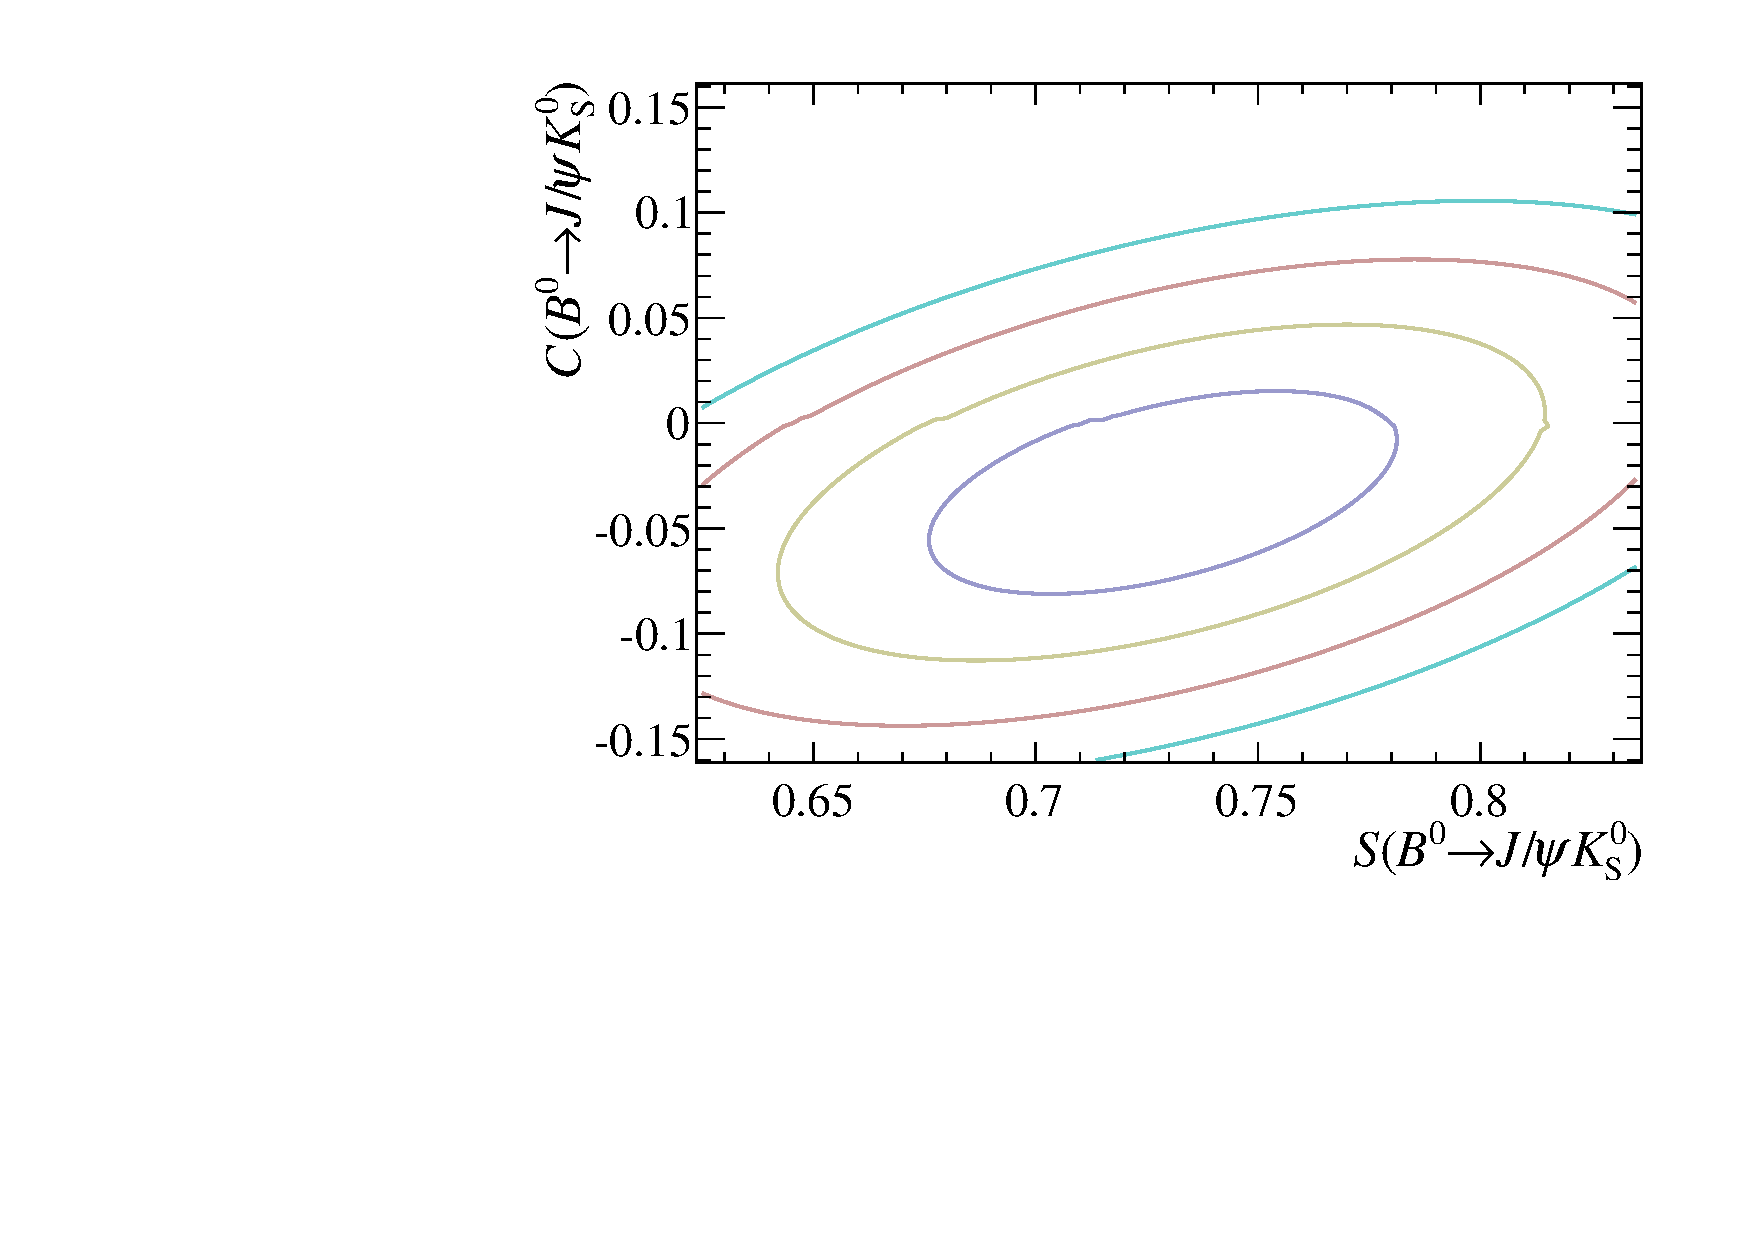
\includegraphics[width=1.00\textwidth]{private/content/measurement-of-sin2beta/figs/LLScan_2D.pdf} \\
  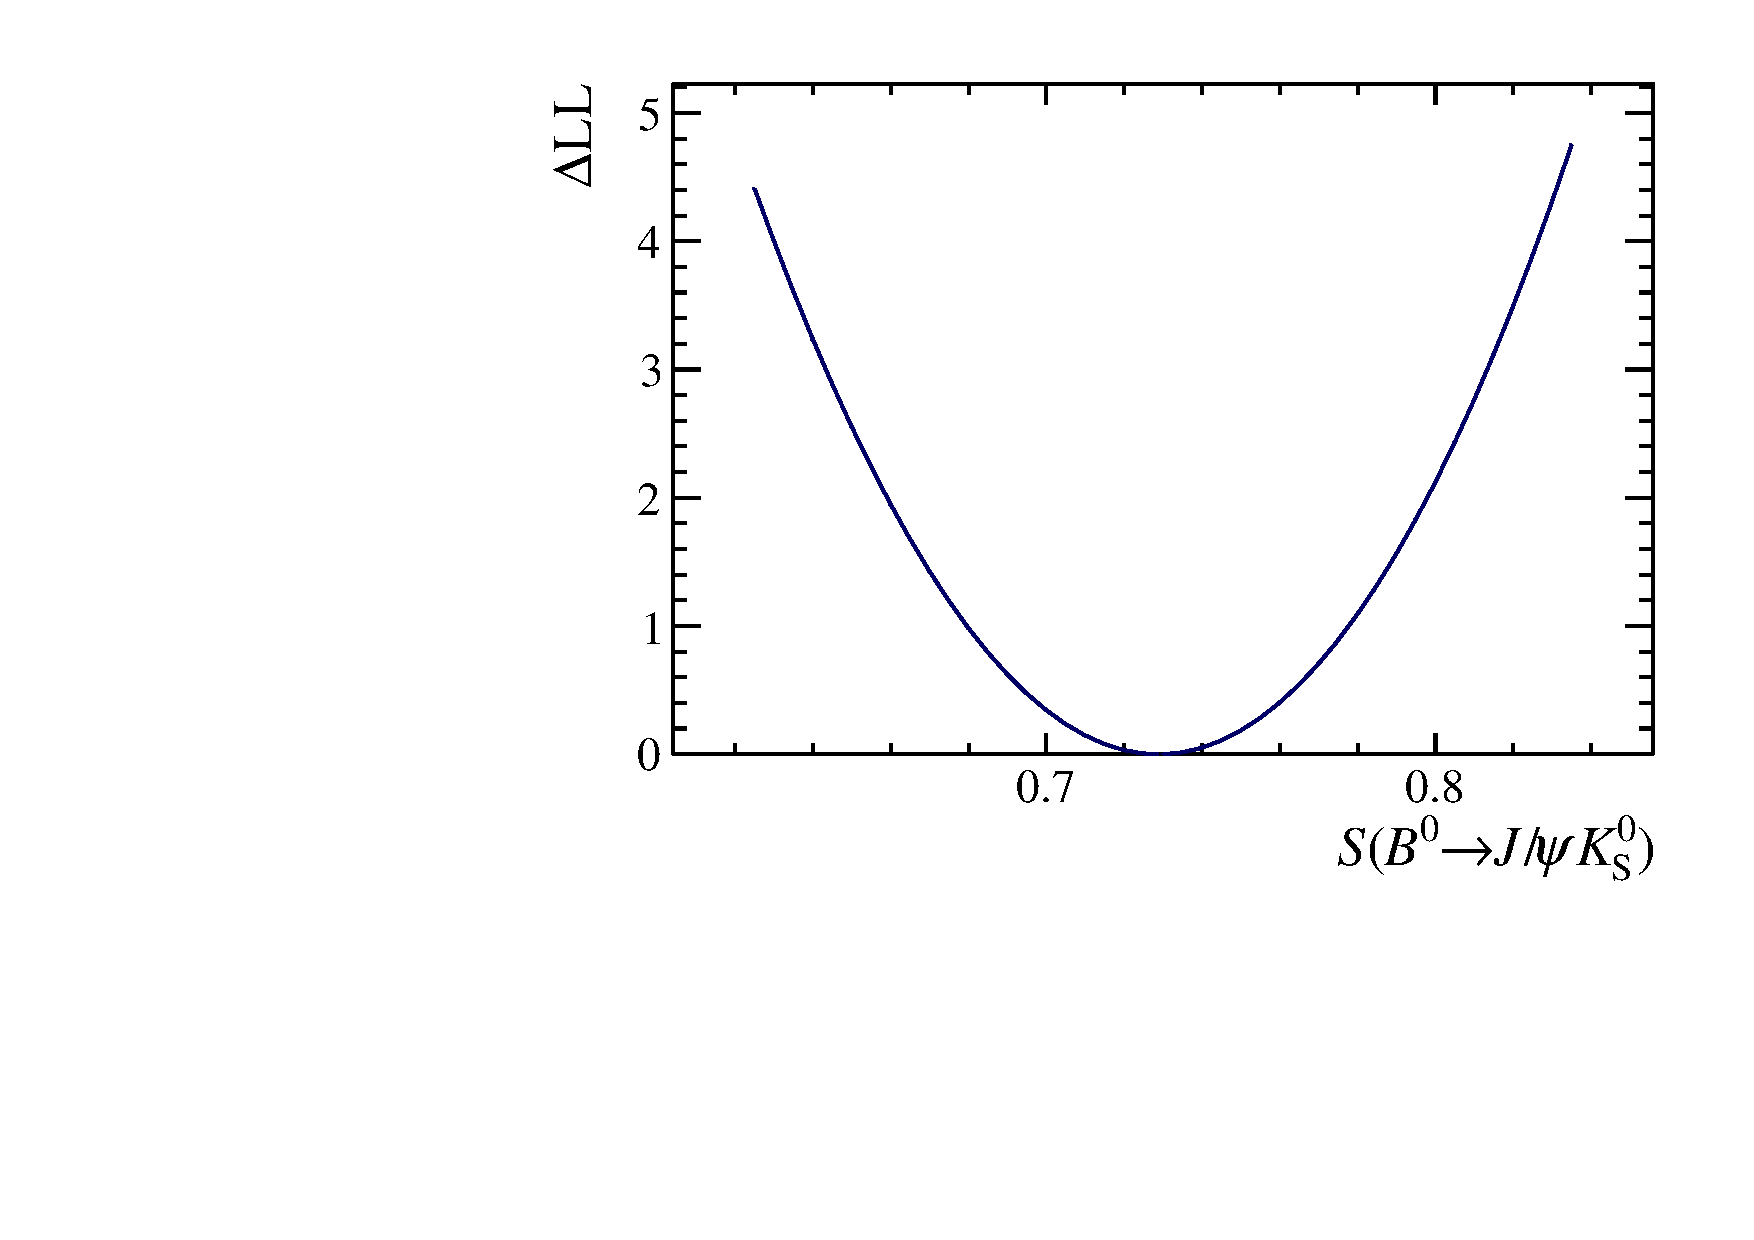
\includegraphics[width=0.46\textwidth]{private/content/measurement-of-sin2beta/figs/LLScan_1D_S.pdf}
  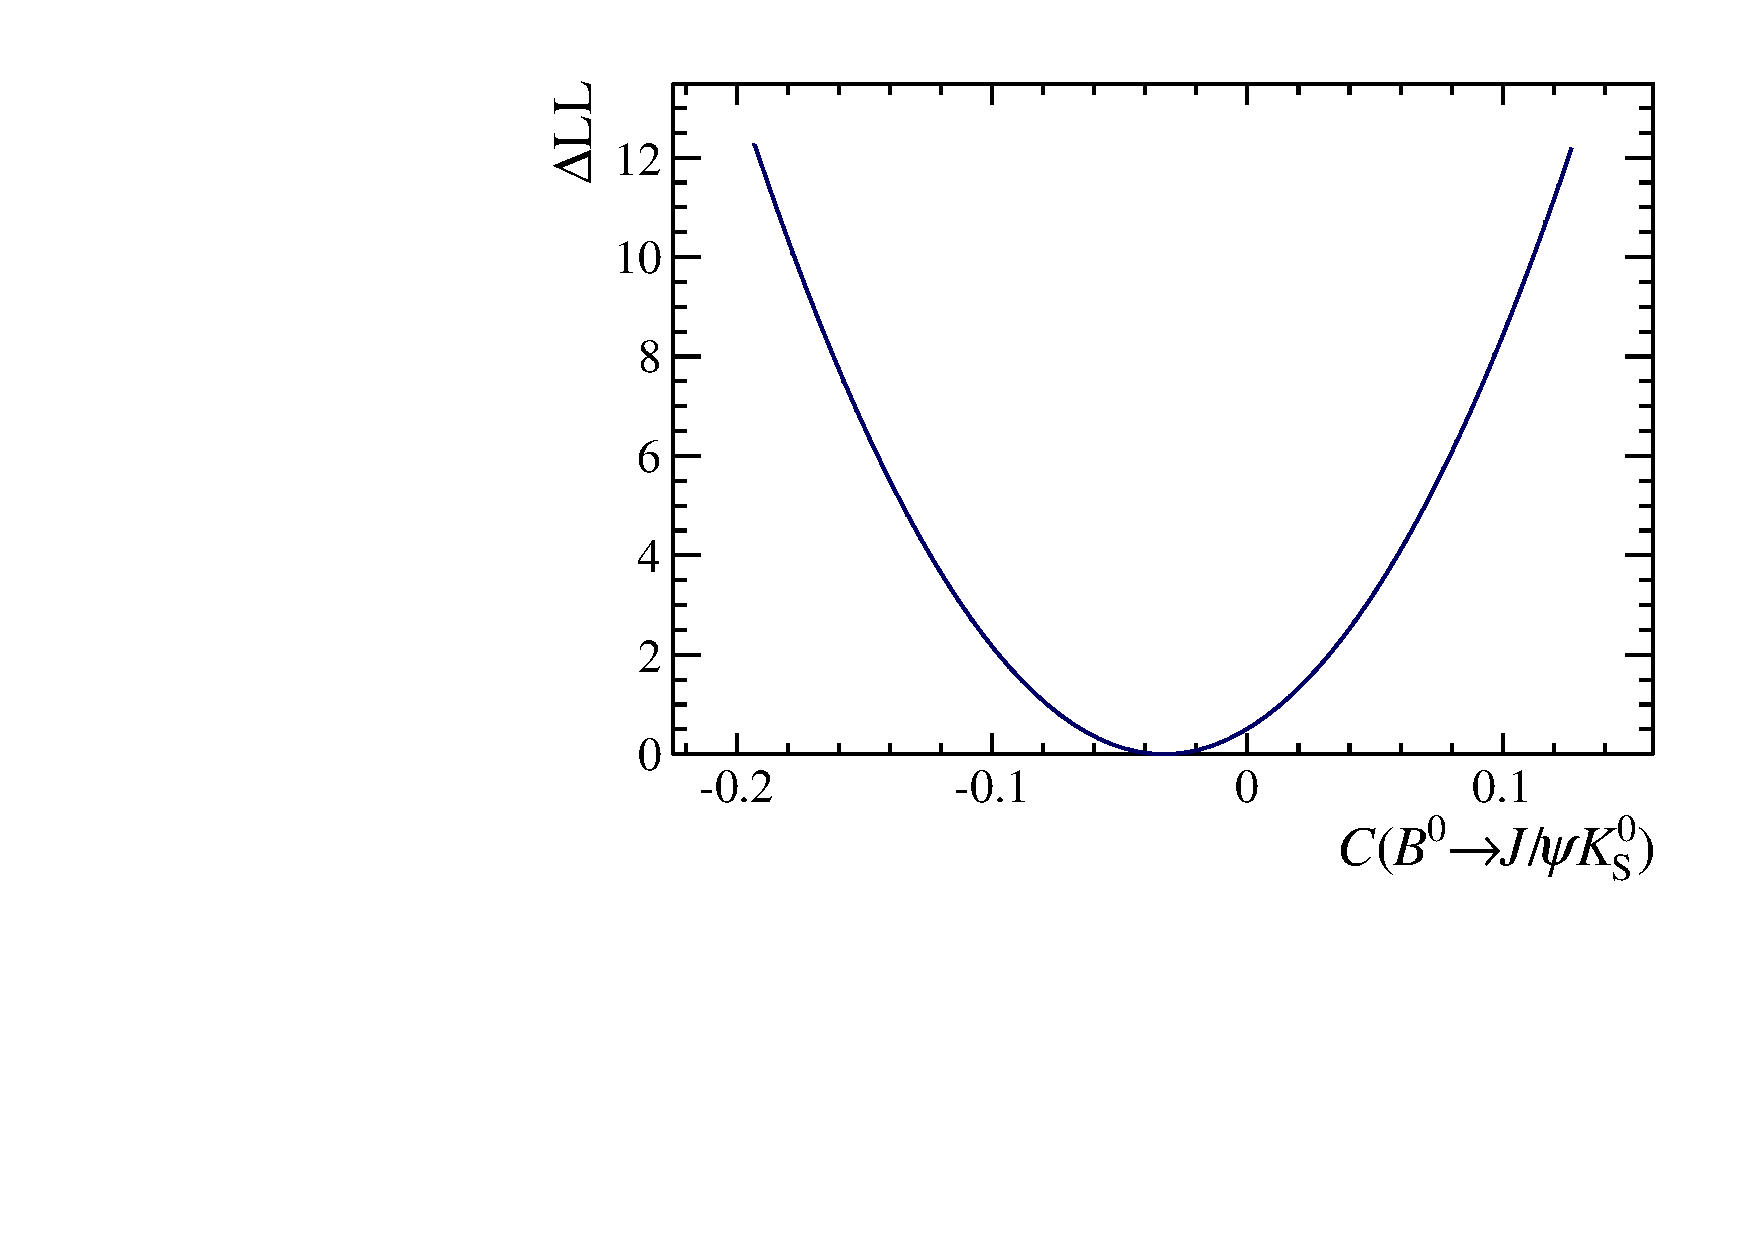
\includegraphics[width=0.46\textwidth]{private/content/measurement-of-sin2beta/figs/LLScan_1D_C.pdf}
  \caption{One and two dimensional likelihood profile scans for $\SJpsiKS$ and $\CJpsiKS$.}
  \label{fig:measurement_of_sin2beta:cpv_measurement:results:plots:ll_scan}
\end{figure}
%
\begin{figure}
\centering
  %!TEX root = ../../../common/main.tex

\pgfdeclareplotmark{cross} {
\pgfpathmoveto{\pgfpoint{-0.3\pgfplotmarksize}{\pgfplotmarksize}}
\pgfpathlineto{\pgfpoint{+0.3\pgfplotmarksize}{\pgfplotmarksize}}
\pgfpathlineto{\pgfpoint{+0.3\pgfplotmarksize}{0.3\pgfplotmarksize}}
\pgfpathlineto{\pgfpoint{+1\pgfplotmarksize}{0.3\pgfplotmarksize}}
\pgfpathlineto{\pgfpoint{+1\pgfplotmarksize}{-0.3\pgfplotmarksize}}
\pgfpathlineto{\pgfpoint{+0.3\pgfplotmarksize}{-0.3\pgfplotmarksize}}
\pgfpathlineto{\pgfpoint{+0.3\pgfplotmarksize}{-1.\pgfplotmarksize}}
\pgfpathlineto{\pgfpoint{-0.3\pgfplotmarksize}{-1.\pgfplotmarksize}}
\pgfpathlineto{\pgfpoint{-0.3\pgfplotmarksize}{-0.3\pgfplotmarksize}}
\pgfpathlineto{\pgfpoint{-1.\pgfplotmarksize}{-0.3\pgfplotmarksize}}
\pgfpathlineto{\pgfpoint{-1.\pgfplotmarksize}{0.3\pgfplotmarksize}}
\pgfpathlineto{\pgfpoint{-0.3\pgfplotmarksize}{0.3\pgfplotmarksize}}
\pgfpathclose
\pgfusepathqstroke
}
\pgfdeclareplotmark{cross*} {
\pgfpathmoveto{\pgfpoint{-0.3\pgfplotmarksize}{\pgfplotmarksize}}
\pgfpathlineto{\pgfpoint{+0.3\pgfplotmarksize}{\pgfplotmarksize}}
\pgfpathlineto{\pgfpoint{+0.3\pgfplotmarksize}{0.3\pgfplotmarksize}}
\pgfpathlineto{\pgfpoint{+1\pgfplotmarksize}{0.3\pgfplotmarksize}}
\pgfpathlineto{\pgfpoint{+1\pgfplotmarksize}{-0.3\pgfplotmarksize}}
\pgfpathlineto{\pgfpoint{+0.3\pgfplotmarksize}{-0.3\pgfplotmarksize}}
\pgfpathlineto{\pgfpoint{+0.3\pgfplotmarksize}{-1.\pgfplotmarksize}}
\pgfpathlineto{\pgfpoint{-0.3\pgfplotmarksize}{-1.\pgfplotmarksize}}
\pgfpathlineto{\pgfpoint{-0.3\pgfplotmarksize}{-0.3\pgfplotmarksize}}
\pgfpathlineto{\pgfpoint{-1.\pgfplotmarksize}{-0.3\pgfplotmarksize}}
\pgfpathlineto{\pgfpoint{-1.\pgfplotmarksize}{0.3\pgfplotmarksize}}
\pgfpathlineto{\pgfpoint{-0.3\pgfplotmarksize}{0.3\pgfplotmarksize}}
\pgfpathclose
\pgfusepathqfillstroke
}
\pgfdeclareplotmark{newstar} {
\pgfpathmoveto{\pgfqpoint{0pt}{\pgfplotmarksize}}
\pgfpathlineto{\pgfqpointpolar{44}{0.5\pgfplotmarksize}}
\pgfpathlineto{\pgfqpointpolar{18}{\pgfplotmarksize}}
\pgfpathlineto{\pgfqpointpolar{-20}{0.5\pgfplotmarksize}}
\pgfpathlineto{\pgfqpointpolar{-54}{\pgfplotmarksize}}
\pgfpathlineto{\pgfqpointpolar{-90}{0.5\pgfplotmarksize}}
\pgfpathlineto{\pgfqpointpolar{234}{\pgfplotmarksize}}
\pgfpathlineto{\pgfqpointpolar{198}{0.5\pgfplotmarksize}}
\pgfpathlineto{\pgfqpointpolar{162}{\pgfplotmarksize}}
\pgfpathlineto{\pgfqpointpolar{134}{0.5\pgfplotmarksize}}
\pgfpathclose
\pgfusepathqstroke
}
\pgfdeclareplotmark{newstar*} {
\pgfpathmoveto{\pgfqpoint{0pt}{\pgfplotmarksize}}
\pgfpathlineto{\pgfqpointpolar{44}{0.5\pgfplotmarksize}}
\pgfpathlineto{\pgfqpointpolar{18}{\pgfplotmarksize}}
\pgfpathlineto{\pgfqpointpolar{-20}{0.5\pgfplotmarksize}}
\pgfpathlineto{\pgfqpointpolar{-54}{\pgfplotmarksize}}
\pgfpathlineto{\pgfqpointpolar{-90}{0.5\pgfplotmarksize}}
\pgfpathlineto{\pgfqpointpolar{234}{\pgfplotmarksize}}
\pgfpathlineto{\pgfqpointpolar{198}{0.5\pgfplotmarksize}}
\pgfpathlineto{\pgfqpointpolar{162}{\pgfplotmarksize}}
\pgfpathlineto{\pgfqpointpolar{134}{0.5\pgfplotmarksize}}
\pgfpathclose
\pgfusepathqfillstroke
}
\begin{tikzpicture}[scale=0.65]
\definecolor{c}{rgb}{1,1,1};
\draw [color=c, fill=c] (0,0) rectangle (20,14.3719);
\draw [color=c, fill=c] (3.23618,2.98992) rectangle (18,13.6533);
\definecolor{c}{rgb}{0,0,0};
\draw [c] (3.23618,2.98992) -- (3.23618,13.6533) -- (18,13.6533) -- (18,2.98992) -- (3.23618,2.98992);
\definecolor{c}{rgb}{1,1,1};
\draw [color=c, fill=c] (3.23618,2.98992) rectangle (18,13.6533);
\definecolor{c}{rgb}{0,0,0};
\draw [c] (3.23618,2.98992) -- (3.23618,13.6533) -- (18,13.6533) -- (18,2.98992) -- (3.23618,2.98992);
\definecolor{c}{rgb}{1,1,1};
\draw [color=c, fill=c] (3.23618,2.98992) rectangle (4.29074,3.75159);
\draw [color=c, fill=c] (4.29074,2.98992) rectangle (5.3453,3.75159);
\draw [color=c, fill=c] (5.3453,2.98992) rectangle (6.39986,3.75159);
\draw [color=c, fill=c] (6.39986,2.98992) rectangle (7.45441,3.75159);
\draw [color=c, fill=c] (7.45441,2.98992) rectangle (8.50897,3.75159);
\draw [color=c, fill=c] (8.50897,2.98992) rectangle (9.56353,3.75159);
\draw [color=c, fill=c] (9.56353,2.98992) rectangle (10.6181,3.75159);
\draw [color=c, fill=c] (10.6181,2.98992) rectangle (11.6726,3.75159);
\draw [color=c, fill=c] (11.6726,2.98992) rectangle (12.7272,3.75159);
\draw [color=c, fill=c] (12.7272,2.98992) rectangle (13.7818,3.75159);
\draw [color=c, fill=c] (13.7818,2.98992) rectangle (14.8363,3.75159);
\draw [color=c, fill=c] (14.8363,2.98992) rectangle (15.8909,3.75159);
\draw [color=c, fill=c] (15.8909,2.98992) rectangle (16.9454,3.75159);
\definecolor{c}{rgb}{0.28,0,0};
\draw [color=c, fill=c] (16.9454,2.98992) rectangle (18,3.75159);
\definecolor{c}{rgb}{0.68,0.68,1};
\draw [color=c, fill=c] (3.23618,3.75159) rectangle (4.29074,4.51326);
\definecolor{c}{rgb}{1,0.866667,0.866667};
\draw [color=c, fill=c] (4.29074,3.75159) rectangle (5.3453,4.51326);
\definecolor{c}{rgb}{1,1,1};
\draw [color=c, fill=c] (5.3453,3.75159) rectangle (6.39986,4.51326);
\draw [color=c, fill=c] (6.39986,3.75159) rectangle (7.45441,4.51326);
\draw [color=c, fill=c] (7.45441,3.75159) rectangle (8.50897,4.51326);
\draw [color=c, fill=c] (8.50897,3.75159) rectangle (9.56353,4.51326);
\draw [color=c, fill=c] (9.56353,3.75159) rectangle (10.6181,4.51326);
\draw [color=c, fill=c] (10.6181,3.75159) rectangle (11.6726,4.51326);
\draw [color=c, fill=c] (11.6726,3.75159) rectangle (12.7272,4.51326);
\draw [color=c, fill=c] (12.7272,3.75159) rectangle (13.7818,4.51326);
\draw [color=c, fill=c] (13.7818,3.75159) rectangle (14.8363,4.51326);
\draw [color=c, fill=c] (14.8363,3.75159) rectangle (15.8909,4.51326);
\definecolor{c}{rgb}{0.28,0,0};
\draw [color=c, fill=c] (15.8909,3.75159) rectangle (16.9454,4.51326);
\definecolor{c}{rgb}{1,1,1};
\draw [color=c, fill=c] (16.9454,3.75159) rectangle (18,4.51326);
\draw [color=c, fill=c] (3.23618,4.51326) rectangle (4.29074,5.27493);
\draw [color=c, fill=c] (4.29074,4.51326) rectangle (5.3453,5.27493);
\draw [color=c, fill=c] (5.3453,4.51326) rectangle (6.39986,5.27493);
\draw [color=c, fill=c] (6.39986,4.51326) rectangle (7.45441,5.27493);
\draw [color=c, fill=c] (7.45441,4.51326) rectangle (8.50897,5.27493);
\draw [color=c, fill=c] (8.50897,4.51326) rectangle (9.56353,5.27493);
\draw [color=c, fill=c] (9.56353,4.51326) rectangle (10.6181,5.27493);
\draw [color=c, fill=c] (10.6181,4.51326) rectangle (11.6726,5.27493);
\draw [color=c, fill=c] (11.6726,4.51326) rectangle (12.7272,5.27493);
\definecolor{c}{rgb}{1,0.733333,0.733333};
\draw [color=c, fill=c] (12.7272,4.51326) rectangle (13.7818,5.27493);
\definecolor{c}{rgb}{1,1,1};
\draw [color=c, fill=c] (13.7818,4.51326) rectangle (14.8363,5.27493);
\definecolor{c}{rgb}{0.28,0,0};
\draw [color=c, fill=c] (14.8363,4.51326) rectangle (15.8909,5.27493);
\definecolor{c}{rgb}{1,1,1};
\draw [color=c, fill=c] (15.8909,4.51326) rectangle (16.9454,5.27493);
\draw [color=c, fill=c] (16.9454,4.51326) rectangle (18,5.27493);
\definecolor{c}{rgb}{0.84,0.84,1};
\draw [color=c, fill=c] (3.23618,5.27493) rectangle (4.29074,6.03659);
\definecolor{c}{rgb}{1,0.866667,0.866667};
\draw [color=c, fill=c] (4.29074,5.27493) rectangle (5.3453,6.03659);
\definecolor{c}{rgb}{1,1,1};
\draw [color=c, fill=c] (5.3453,5.27493) rectangle (6.39986,6.03659);
\draw [color=c, fill=c] (6.39986,5.27493) rectangle (7.45441,6.03659);
\draw [color=c, fill=c] (7.45441,5.27493) rectangle (8.50897,6.03659);
\draw [color=c, fill=c] (8.50897,5.27493) rectangle (9.56353,6.03659);
\draw [color=c, fill=c] (9.56353,5.27493) rectangle (10.6181,6.03659);
\draw [color=c, fill=c] (10.6181,5.27493) rectangle (11.6726,6.03659);
\definecolor{c}{rgb}{1,0.733333,0.733333};
\draw [color=c, fill=c] (11.6726,5.27493) rectangle (12.7272,6.03659);
\definecolor{c}{rgb}{1,1,1};
\draw [color=c, fill=c] (12.7272,5.27493) rectangle (13.7818,6.03659);
\definecolor{c}{rgb}{0.28,0,0};
\draw [color=c, fill=c] (13.7818,5.27493) rectangle (14.8363,6.03659);
\definecolor{c}{rgb}{1,1,1};
\draw [color=c, fill=c] (14.8363,5.27493) rectangle (15.8909,6.03659);
\draw [color=c, fill=c] (15.8909,5.27493) rectangle (16.9454,6.03659);
\draw [color=c, fill=c] (16.9454,5.27493) rectangle (18,6.03659);
\draw [color=c, fill=c] (3.23618,6.03659) rectangle (4.29074,6.79826);
\draw [color=c, fill=c] (4.29074,6.03659) rectangle (5.3453,6.79826);
\draw [color=c, fill=c] (5.3453,6.03659) rectangle (6.39986,6.79826);
\draw [color=c, fill=c] (6.39986,6.03659) rectangle (7.45441,6.79826);
\draw [color=c, fill=c] (7.45441,6.03659) rectangle (8.50897,6.79826);
\draw [color=c, fill=c] (8.50897,6.03659) rectangle (9.56353,6.79826);
\draw [color=c, fill=c] (9.56353,6.03659) rectangle (10.6181,6.79826);
\draw [color=c, fill=c] (10.6181,6.03659) rectangle (11.6726,6.79826);
\draw [color=c, fill=c] (11.6726,6.03659) rectangle (12.7272,6.79826);
\definecolor{c}{rgb}{0.28,0,0};
\draw [color=c, fill=c] (12.7272,6.03659) rectangle (13.7818,6.79826);
\definecolor{c}{rgb}{1,1,1};
\draw [color=c, fill=c] (13.7818,6.03659) rectangle (14.8363,6.79826);
\definecolor{c}{rgb}{1,0.733333,0.733333};
\draw [color=c, fill=c] (14.8363,6.03659) rectangle (15.8909,6.79826);
\definecolor{c}{rgb}{1,1,1};
\draw [color=c, fill=c] (15.8909,6.03659) rectangle (16.9454,6.79826);
\draw [color=c, fill=c] (16.9454,6.03659) rectangle (18,6.79826);
\definecolor{c}{rgb}{1,0.866667,0.866667};
\draw [color=c, fill=c] (3.23618,6.79826) rectangle (4.29074,7.55993);
\definecolor{c}{rgb}{1,1,1};
\draw [color=c, fill=c] (4.29074,6.79826) rectangle (5.3453,7.55993);
\draw [color=c, fill=c] (5.3453,6.79826) rectangle (6.39986,7.55993);
\draw [color=c, fill=c] (6.39986,6.79826) rectangle (7.45441,7.55993);
\draw [color=c, fill=c] (7.45441,6.79826) rectangle (8.50897,7.55993);
\draw [color=c, fill=c] (8.50897,6.79826) rectangle (9.56353,7.55993);
\draw [color=c, fill=c] (9.56353,6.79826) rectangle (10.6181,7.55993);
\draw [color=c, fill=c] (10.6181,6.79826) rectangle (11.6726,7.55993);
\definecolor{c}{rgb}{0.28,0,0};
\draw [color=c, fill=c] (11.6726,6.79826) rectangle (12.7272,7.55993);
\definecolor{c}{rgb}{1,1,1};
\draw [color=c, fill=c] (12.7272,6.79826) rectangle (13.7818,7.55993);
\definecolor{c}{rgb}{1,0.733333,0.733333};
\draw [color=c, fill=c] (13.7818,6.79826) rectangle (14.8363,7.55993);
\definecolor{c}{rgb}{1,1,1};
\draw [color=c, fill=c] (14.8363,6.79826) rectangle (15.8909,7.55993);
\draw [color=c, fill=c] (15.8909,6.79826) rectangle (16.9454,7.55993);
\draw [color=c, fill=c] (16.9454,6.79826) rectangle (18,7.55993);
\definecolor{c}{rgb}{1,0.866667,0.866667};
\draw [color=c, fill=c] (3.23618,7.55993) rectangle (4.29074,8.3216);
\definecolor{c}{rgb}{1,1,1};
\draw [color=c, fill=c] (4.29074,7.55993) rectangle (5.3453,8.3216);
\draw [color=c, fill=c] (5.3453,7.55993) rectangle (6.39986,8.3216);
\draw [color=c, fill=c] (6.39986,7.55993) rectangle (7.45441,8.3216);
\draw [color=c, fill=c] (7.45441,7.55993) rectangle (8.50897,8.3216);
\draw [color=c, fill=c] (8.50897,7.55993) rectangle (9.56353,8.3216);
\definecolor{c}{rgb}{1,0.733333,0.733333};
\draw [color=c, fill=c] (9.56353,7.55993) rectangle (10.6181,8.3216);
\definecolor{c}{rgb}{0.28,0,0};
\draw [color=c, fill=c] (10.6181,7.55993) rectangle (11.6726,8.3216);
\definecolor{c}{rgb}{1,1,1};
\draw [color=c, fill=c] (11.6726,7.55993) rectangle (12.7272,8.3216);
\draw [color=c, fill=c] (12.7272,7.55993) rectangle (13.7818,8.3216);
\draw [color=c, fill=c] (13.7818,7.55993) rectangle (14.8363,8.3216);
\draw [color=c, fill=c] (14.8363,7.55993) rectangle (15.8909,8.3216);
\draw [color=c, fill=c] (15.8909,7.55993) rectangle (16.9454,8.3216);
\draw [color=c, fill=c] (16.9454,7.55993) rectangle (18,8.3216);
\definecolor{c}{rgb}{0.84,0.84,1};
\draw [color=c, fill=c] (3.23618,8.3216) rectangle (4.29074,9.08326);
\definecolor{c}{rgb}{1,1,1};
\draw [color=c, fill=c] (4.29074,8.3216) rectangle (5.3453,9.08326);
\draw [color=c, fill=c] (5.3453,8.3216) rectangle (6.39986,9.08326);
\draw [color=c, fill=c] (6.39986,8.3216) rectangle (7.45441,9.08326);
\draw [color=c, fill=c] (7.45441,8.3216) rectangle (8.50897,9.08326);
\draw [color=c, fill=c] (8.50897,8.3216) rectangle (9.56353,9.08326);
\definecolor{c}{rgb}{0.28,0,0};
\draw [color=c, fill=c] (9.56353,8.3216) rectangle (10.6181,9.08326);
\definecolor{c}{rgb}{1,0.733333,0.733333};
\draw [color=c, fill=c] (10.6181,8.3216) rectangle (11.6726,9.08326);
\definecolor{c}{rgb}{1,1,1};
\draw [color=c, fill=c] (11.6726,8.3216) rectangle (12.7272,9.08326);
\draw [color=c, fill=c] (12.7272,8.3216) rectangle (13.7818,9.08326);
\draw [color=c, fill=c] (13.7818,8.3216) rectangle (14.8363,9.08326);
\draw [color=c, fill=c] (14.8363,8.3216) rectangle (15.8909,9.08326);
\draw [color=c, fill=c] (15.8909,8.3216) rectangle (16.9454,9.08326);
\draw [color=c, fill=c] (16.9454,8.3216) rectangle (18,9.08326);
\definecolor{c}{rgb}{0.84,0.84,1};
\draw [color=c, fill=c] (3.23618,9.08326) rectangle (4.29074,9.84493);
\definecolor{c}{rgb}{1,1,1};
\draw [color=c, fill=c] (4.29074,9.08326) rectangle (5.3453,9.84493);
\draw [color=c, fill=c] (5.3453,9.08326) rectangle (6.39986,9.84493);
\draw [color=c, fill=c] (6.39986,9.08326) rectangle (7.45441,9.84493);
\definecolor{c}{rgb}{1,0.733333,0.733333};
\draw [color=c, fill=c] (7.45441,9.08326) rectangle (8.50897,9.84493);
\definecolor{c}{rgb}{0.28,0,0};
\draw [color=c, fill=c] (8.50897,9.08326) rectangle (9.56353,9.84493);
\definecolor{c}{rgb}{1,1,1};
\draw [color=c, fill=c] (9.56353,9.08326) rectangle (10.6181,9.84493);
\draw [color=c, fill=c] (10.6181,9.08326) rectangle (11.6726,9.84493);
\draw [color=c, fill=c] (11.6726,9.08326) rectangle (12.7272,9.84493);
\draw [color=c, fill=c] (12.7272,9.08326) rectangle (13.7818,9.84493);
\draw [color=c, fill=c] (13.7818,9.08326) rectangle (14.8363,9.84493);
\draw [color=c, fill=c] (14.8363,9.08326) rectangle (15.8909,9.84493);
\draw [color=c, fill=c] (15.8909,9.08326) rectangle (16.9454,9.84493);
\draw [color=c, fill=c] (16.9454,9.08326) rectangle (18,9.84493);
\definecolor{c}{rgb}{1,0.866667,0.866667};
\draw [color=c, fill=c] (3.23618,9.84493) rectangle (4.29074,10.6066);
\definecolor{c}{rgb}{1,1,1};
\draw [color=c, fill=c] (4.29074,9.84493) rectangle (5.3453,10.6066);
\draw [color=c, fill=c] (5.3453,9.84493) rectangle (6.39986,10.6066);
\draw [color=c, fill=c] (6.39986,9.84493) rectangle (7.45441,10.6066);
\definecolor{c}{rgb}{0.28,0,0};
\draw [color=c, fill=c] (7.45441,9.84493) rectangle (8.50897,10.6066);
\definecolor{c}{rgb}{1,0.733333,0.733333};
\draw [color=c, fill=c] (8.50897,9.84493) rectangle (9.56353,10.6066);
\definecolor{c}{rgb}{1,1,1};
\draw [color=c, fill=c] (9.56353,9.84493) rectangle (10.6181,10.6066);
\draw [color=c, fill=c] (10.6181,9.84493) rectangle (11.6726,10.6066);
\draw [color=c, fill=c] (11.6726,9.84493) rectangle (12.7272,10.6066);
\draw [color=c, fill=c] (12.7272,9.84493) rectangle (13.7818,10.6066);
\draw [color=c, fill=c] (13.7818,9.84493) rectangle (14.8363,10.6066);
\draw [color=c, fill=c] (14.8363,9.84493) rectangle (15.8909,10.6066);
\draw [color=c, fill=c] (15.8909,9.84493) rectangle (16.9454,10.6066);
\draw [color=c, fill=c] (16.9454,9.84493) rectangle (18,10.6066);
\draw [color=c, fill=c] (3.23618,10.6066) rectangle (4.29074,11.3683);
\draw [color=c, fill=c] (4.29074,10.6066) rectangle (5.3453,11.3683);
\draw [color=c, fill=c] (5.3453,10.6066) rectangle (6.39986,11.3683);
\definecolor{c}{rgb}{0.28,0,0};
\draw [color=c, fill=c] (6.39986,10.6066) rectangle (7.45441,11.3683);
\definecolor{c}{rgb}{1,1,1};
\draw [color=c, fill=c] (7.45441,10.6066) rectangle (8.50897,11.3683);
\draw [color=c, fill=c] (8.50897,10.6066) rectangle (9.56353,11.3683);
\draw [color=c, fill=c] (9.56353,10.6066) rectangle (10.6181,11.3683);
\draw [color=c, fill=c] (10.6181,10.6066) rectangle (11.6726,11.3683);
\draw [color=c, fill=c] (11.6726,10.6066) rectangle (12.7272,11.3683);
\draw [color=c, fill=c] (12.7272,10.6066) rectangle (13.7818,11.3683);
\draw [color=c, fill=c] (13.7818,10.6066) rectangle (14.8363,11.3683);
\draw [color=c, fill=c] (14.8363,10.6066) rectangle (15.8909,11.3683);
\draw [color=c, fill=c] (15.8909,10.6066) rectangle (16.9454,11.3683);
\draw [color=c, fill=c] (16.9454,10.6066) rectangle (18,11.3683);
\draw [color=c, fill=c] (3.23618,11.3683) rectangle (4.29074,12.1299);
\draw [color=c, fill=c] (4.29074,11.3683) rectangle (5.3453,12.1299);
\definecolor{c}{rgb}{0.28,0,0};
\draw [color=c, fill=c] (5.3453,11.3683) rectangle (6.39986,12.1299);
\definecolor{c}{rgb}{1,1,1};
\draw [color=c, fill=c] (6.39986,11.3683) rectangle (7.45441,12.1299);
\draw [color=c, fill=c] (7.45441,11.3683) rectangle (8.50897,12.1299);
\draw [color=c, fill=c] (8.50897,11.3683) rectangle (9.56353,12.1299);
\draw [color=c, fill=c] (9.56353,11.3683) rectangle (10.6181,12.1299);
\draw [color=c, fill=c] (10.6181,11.3683) rectangle (11.6726,12.1299);
\draw [color=c, fill=c] (11.6726,11.3683) rectangle (12.7272,12.1299);
\draw [color=c, fill=c] (12.7272,11.3683) rectangle (13.7818,12.1299);
\draw [color=c, fill=c] (13.7818,11.3683) rectangle (14.8363,12.1299);
\draw [color=c, fill=c] (14.8363,11.3683) rectangle (15.8909,12.1299);
\draw [color=c, fill=c] (15.8909,11.3683) rectangle (16.9454,12.1299);
\draw [color=c, fill=c] (16.9454,11.3683) rectangle (18,12.1299);
\definecolor{c}{rgb}{1,0.05,0.05};
\draw [color=c, fill=c] (3.23618,12.1299) rectangle (4.29074,12.8916);
\definecolor{c}{rgb}{0.28,0,0};
\draw [color=c, fill=c] (4.29074,12.1299) rectangle (5.3453,12.8916);
\definecolor{c}{rgb}{1,1,1};
\draw [color=c, fill=c] (5.3453,12.1299) rectangle (6.39986,12.8916);
\draw [color=c, fill=c] (6.39986,12.1299) rectangle (7.45441,12.8916);
\draw [color=c, fill=c] (7.45441,12.1299) rectangle (8.50897,12.8916);
\draw [color=c, fill=c] (8.50897,12.1299) rectangle (9.56353,12.8916);
\draw [color=c, fill=c] (9.56353,12.1299) rectangle (10.6181,12.8916);
\draw [color=c, fill=c] (10.6181,12.1299) rectangle (11.6726,12.8916);
\draw [color=c, fill=c] (11.6726,12.1299) rectangle (12.7272,12.8916);
\draw [color=c, fill=c] (12.7272,12.1299) rectangle (13.7818,12.8916);
\definecolor{c}{rgb}{1,0.866667,0.866667};
\draw [color=c, fill=c] (13.7818,12.1299) rectangle (14.8363,12.8916);
\definecolor{c}{rgb}{1,1,1};
\draw [color=c, fill=c] (14.8363,12.1299) rectangle (15.8909,12.8916);
\definecolor{c}{rgb}{1,0.866667,0.866667};
\draw [color=c, fill=c] (15.8909,12.1299) rectangle (16.9454,12.8916);
\definecolor{c}{rgb}{1,1,1};
\draw [color=c, fill=c] (16.9454,12.1299) rectangle (18,12.8916);
\definecolor{c}{rgb}{0.28,0,0};
\draw [color=c, fill=c] (3.23618,12.8916) rectangle (4.29074,13.6533);
\definecolor{c}{rgb}{1,0.05,0.05};
\draw [color=c, fill=c] (4.29074,12.8916) rectangle (5.3453,13.6533);
\definecolor{c}{rgb}{1,1,1};
\draw [color=c, fill=c] (5.3453,12.8916) rectangle (6.39986,13.6533);
\draw [color=c, fill=c] (6.39986,12.8916) rectangle (7.45441,13.6533);
\definecolor{c}{rgb}{1,0.866667,0.866667};
\draw [color=c, fill=c] (7.45441,12.8916) rectangle (8.50897,13.6533);
\definecolor{c}{rgb}{0.84,0.84,1};
\draw [color=c, fill=c] (8.50897,12.8916) rectangle (9.56353,13.6533);
\draw [color=c, fill=c] (9.56353,12.8916) rectangle (10.6181,13.6533);
\definecolor{c}{rgb}{1,0.866667,0.866667};
\draw [color=c, fill=c] (10.6181,12.8916) rectangle (11.6726,13.6533);
\draw [color=c, fill=c] (11.6726,12.8916) rectangle (12.7272,13.6533);
\definecolor{c}{rgb}{1,1,1};
\draw [color=c, fill=c] (12.7272,12.8916) rectangle (13.7818,13.6533);
\definecolor{c}{rgb}{0.84,0.84,1};
\draw [color=c, fill=c] (13.7818,12.8916) rectangle (14.8363,13.6533);
\definecolor{c}{rgb}{1,1,1};
\draw [color=c, fill=c] (14.8363,12.8916) rectangle (15.8909,13.6533);
\definecolor{c}{rgb}{0.68,0.68,1};
\draw [color=c, fill=c] (15.8909,12.8916) rectangle (16.9454,13.6533);
\definecolor{c}{rgb}{1,1,1};
\draw [color=c, fill=c] (16.9454,12.8916) rectangle (18,13.6533);
\draw (3.76346,3.37076) node[scale=0.766067, rotate=0]{-0.0};
\draw (4.81802,3.37076) node[scale=0.766067, rotate=0]{0.0};
\draw (5.87258,3.37076) node[scale=0.766067, rotate=0]{-0.0};
\draw (6.92714,3.37076) node[scale=0.766067, rotate=0]{-0.0};
\draw (7.98169,3.37076) node[scale=0.766067, rotate=0]{-0.0};
\draw (9.03625,3.37076) node[scale=0.766067, rotate=0]{0.0};
\draw (10.0908,3.37076) node[scale=0.766067, rotate=0]{-0.0};
\draw (11.1454,3.37076) node[scale=0.766067, rotate=0]{-0.0};
\draw (12.1999,3.37076) node[scale=0.766067, rotate=0]{-0.0};
\draw (13.2545,3.37076) node[scale=0.766067, rotate=0]{-0.0};
\draw (14.309,3.37076) node[scale=0.766067, rotate=0]{-0.0};
\draw (15.3636,3.37076) node[scale=0.766067, rotate=0]{0.0};
\draw (16.4182,3.37076) node[scale=0.766067, rotate=0]{-0.0};
\draw (17.4727,3.37076) node[scale=0.766067, rotate=0]{1.0};
\draw (3.76346,4.13243) node[scale=0.766067, rotate=0]{-0.1};
\draw (4.81802,4.13243) node[scale=0.766067, rotate=0]{0.1};
\draw (5.87258,4.13243) node[scale=0.766067, rotate=0]{-0.0};
\draw (6.92714,4.13243) node[scale=0.766067, rotate=0]{-0.0};
\draw (7.98169,4.13243) node[scale=0.766067, rotate=0]{-0.0};
\draw (9.03625,4.13243) node[scale=0.766067, rotate=0]{0.0};
\draw (10.0908,4.13243) node[scale=0.766067, rotate=0]{-0.0};
\draw (11.1454,4.13243) node[scale=0.766067, rotate=0]{0.0};
\draw (12.1999,4.13243) node[scale=0.766067, rotate=0]{-0.0};
\draw (13.2545,4.13243) node[scale=0.766067, rotate=0]{-0.0};
\draw (14.309,4.13243) node[scale=0.766067, rotate=0]{-0.0};
\draw (15.3636,4.13243) node[scale=0.766067, rotate=0]{0.0};
\draw (16.4182,4.13243) node[scale=0.766067, rotate=0]{1.0};
\draw (17.4727,4.13243) node[scale=0.766067, rotate=0]{-0.0};
\draw (3.76346,4.89409) node[scale=0.766067, rotate=0]{0.0};
\draw (4.81802,4.89409) node[scale=0.766067, rotate=0]{-0.0};
\draw (5.87258,4.89409) node[scale=0.766067, rotate=0]{-0.0};
\draw (6.92714,4.89409) node[scale=0.766067, rotate=0]{0.0};
\draw (7.98169,4.89409) node[scale=0.766067, rotate=0]{0.0};
\draw (9.03625,4.89409) node[scale=0.766067, rotate=0]{-0.0};
\draw (10.0908,4.89409) node[scale=0.766067, rotate=0]{-0.0};
\draw (11.1454,4.89409) node[scale=0.766067, rotate=0]{0.0};
\draw (12.1999,4.89409) node[scale=0.766067, rotate=0]{0.0};
\draw (13.2545,4.89409) node[scale=0.766067, rotate=0]{0.1};
\draw (14.309,4.89409) node[scale=0.766067, rotate=0]{0.0};
\draw (15.3636,4.89409) node[scale=0.766067, rotate=0]{1.0};
\draw (16.4182,4.89409) node[scale=0.766067, rotate=0]{0.0};
\draw (17.4727,4.89409) node[scale=0.766067, rotate=0]{0.0};
\draw (3.76346,5.65576) node[scale=0.766067, rotate=0]{-0.1};
\draw (4.81802,5.65576) node[scale=0.766067, rotate=0]{0.0};
\draw (5.87258,5.65576) node[scale=0.766067, rotate=0]{0.0};
\draw (6.92714,5.65576) node[scale=0.766067, rotate=0]{-0.0};
\draw (7.98169,5.65576) node[scale=0.766067, rotate=0]{-0.0};
\draw (9.03625,5.65576) node[scale=0.766067, rotate=0]{0.0};
\draw (10.0908,5.65576) node[scale=0.766067, rotate=0]{0.0};
\draw (11.1454,5.65576) node[scale=0.766067, rotate=0]{-0.0};
\draw (12.1999,5.65576) node[scale=0.766067, rotate=0]{0.1};
\draw (13.2545,5.65576) node[scale=0.766067, rotate=0]{0.0};
\draw (14.309,5.65576) node[scale=0.766067, rotate=0]{1.0};
\draw (15.3636,5.65576) node[scale=0.766067, rotate=0]{0.0};
\draw (16.4182,5.65576) node[scale=0.766067, rotate=0]{-0.0};
\draw (17.4727,5.65576) node[scale=0.766067, rotate=0]{-0.0};
\draw (3.76346,6.41743) node[scale=0.766067, rotate=0]{-0.0};
\draw (4.81802,6.41743) node[scale=0.766067, rotate=0]{0.0};
\draw (5.87258,6.41743) node[scale=0.766067, rotate=0]{0.0};
\draw (6.92714,6.41743) node[scale=0.766067, rotate=0]{0.0};
\draw (7.98169,6.41743) node[scale=0.766067, rotate=0]{-0.0};
\draw (9.03625,6.41743) node[scale=0.766067, rotate=0]{0.0};
\draw (10.0908,6.41743) node[scale=0.766067, rotate=0]{0.0};
\draw (11.1454,6.41743) node[scale=0.766067, rotate=0]{-0.0};
\draw (12.1999,6.41743) node[scale=0.766067, rotate=0]{0.0};
\draw (13.2545,6.41743) node[scale=0.766067, rotate=0]{1.0};
\draw (14.309,6.41743) node[scale=0.766067, rotate=0]{0.0};
\draw (15.3636,6.41743) node[scale=0.766067, rotate=0]{0.1};
\draw (16.4182,6.41743) node[scale=0.766067, rotate=0]{-0.0};
\draw (17.4727,6.41743) node[scale=0.766067, rotate=0]{-0.0};
\draw (3.76346,7.17909) node[scale=0.766067, rotate=0]{0.1};
\draw (4.81802,7.17909) node[scale=0.766067, rotate=0]{0.0};
\draw (5.87258,7.17909) node[scale=0.766067, rotate=0]{0.0};
\draw (6.92714,7.17909) node[scale=0.766067, rotate=0]{0.0};
\draw (7.98169,7.17909) node[scale=0.766067, rotate=0]{0.0};
\draw (9.03625,7.17909) node[scale=0.766067, rotate=0]{-0.0};
\draw (10.0908,7.17909) node[scale=0.766067, rotate=0]{-0.0};
\draw (11.1454,7.17909) node[scale=0.766067, rotate=0]{0.0};
\draw (12.1999,7.17909) node[scale=0.766067, rotate=0]{1.0};
\draw (13.2545,7.17909) node[scale=0.766067, rotate=0]{0.0};
\draw (14.309,7.17909) node[scale=0.766067, rotate=0]{0.1};
\draw (15.3636,7.17909) node[scale=0.766067, rotate=0]{0.0};
\draw (16.4182,7.17909) node[scale=0.766067, rotate=0]{-0.0};
\draw (17.4727,7.17909) node[scale=0.766067, rotate=0]{-0.0};
\draw (3.76346,7.94076) node[scale=0.766067, rotate=0]{0.1};
\draw (4.81802,7.94076) node[scale=0.766067, rotate=0]{-0.0};
\draw (5.87258,7.94076) node[scale=0.766067, rotate=0]{-0.0};
\draw (6.92714,7.94076) node[scale=0.766067, rotate=0]{0.0};
\draw (7.98169,7.94076) node[scale=0.766067, rotate=0]{0.0};
\draw (9.03625,7.94076) node[scale=0.766067, rotate=0]{0.0};
\draw (10.0908,7.94076) node[scale=0.766067, rotate=0]{0.1};
\draw (11.1454,7.94076) node[scale=0.766067, rotate=0]{1.0};
\draw (12.1999,7.94076) node[scale=0.766067, rotate=0]{0.0};
\draw (13.2545,7.94076) node[scale=0.766067, rotate=0]{-0.0};
\draw (14.309,7.94076) node[scale=0.766067, rotate=0]{-0.0};
\draw (15.3636,7.94076) node[scale=0.766067, rotate=0]{0.0};
\draw (16.4182,7.94076) node[scale=0.766067, rotate=0]{0.0};
\draw (17.4727,7.94076) node[scale=0.766067, rotate=0]{-0.0};
\draw (3.76346,8.70243) node[scale=0.766067, rotate=0]{-0.1};
\draw (4.81802,8.70243) node[scale=0.766067, rotate=0]{0.0};
\draw (5.87258,8.70243) node[scale=0.766067, rotate=0]{0.0};
\draw (6.92714,8.70243) node[scale=0.766067, rotate=0]{-0.0};
\draw (7.98169,8.70243) node[scale=0.766067, rotate=0]{0.0};
\draw (9.03625,8.70243) node[scale=0.766067, rotate=0]{0.0};
\draw (10.0908,8.70243) node[scale=0.766067, rotate=0]{1.0};
\draw (11.1454,8.70243) node[scale=0.766067, rotate=0]{0.1};
\draw (12.1999,8.70243) node[scale=0.766067, rotate=0]{-0.0};
\draw (13.2545,8.70243) node[scale=0.766067, rotate=0]{0.0};
\draw (14.309,8.70243) node[scale=0.766067, rotate=0]{0.0};
\draw (15.3636,8.70243) node[scale=0.766067, rotate=0]{-0.0};
\draw (16.4182,8.70243) node[scale=0.766067, rotate=0]{-0.0};
\draw (17.4727,8.70243) node[scale=0.766067, rotate=0]{-0.0};
\draw (3.76346,9.4641) node[scale=0.766067, rotate=0]{-0.1};
\draw (4.81802,9.4641) node[scale=0.766067, rotate=0]{0.0};
\draw (5.87258,9.4641) node[scale=0.766067, rotate=0]{-0.0};
\draw (6.92714,9.4641) node[scale=0.766067, rotate=0]{-0.0};
\draw (7.98169,9.4641) node[scale=0.766067, rotate=0]{0.1};
\draw (9.03625,9.4641) node[scale=0.766067, rotate=0]{1.0};
\draw (10.0908,9.4641) node[scale=0.766067, rotate=0]{0.0};
\draw (11.1454,9.4641) node[scale=0.766067, rotate=0]{0.0};
\draw (12.1999,9.4641) node[scale=0.766067, rotate=0]{-0.0};
\draw (13.2545,9.4641) node[scale=0.766067, rotate=0]{0.0};
\draw (14.309,9.4641) node[scale=0.766067, rotate=0]{0.0};
\draw (15.3636,9.4641) node[scale=0.766067, rotate=0]{-0.0};
\draw (16.4182,9.4641) node[scale=0.766067, rotate=0]{0.0};
\draw (17.4727,9.4641) node[scale=0.766067, rotate=0]{0.0};
\draw (3.76346,10.2258) node[scale=0.766067, rotate=0]{0.1};
\draw (4.81802,10.2258) node[scale=0.766067, rotate=0]{-0.0};
\draw (5.87258,10.2258) node[scale=0.766067, rotate=0]{0.0};
\draw (6.92714,10.2258) node[scale=0.766067, rotate=0]{-0.0};
\draw (7.98169,10.2258) node[scale=0.766067, rotate=0]{1.0};
\draw (9.03625,10.2258) node[scale=0.766067, rotate=0]{0.1};
\draw (10.0908,10.2258) node[scale=0.766067, rotate=0]{0.0};
\draw (11.1454,10.2258) node[scale=0.766067, rotate=0]{0.0};
\draw (12.1999,10.2258) node[scale=0.766067, rotate=0]{0.0};
\draw (13.2545,10.2258) node[scale=0.766067, rotate=0]{-0.0};
\draw (14.309,10.2258) node[scale=0.766067, rotate=0]{-0.0};
\draw (15.3636,10.2258) node[scale=0.766067, rotate=0]{0.0};
\draw (16.4182,10.2258) node[scale=0.766067, rotate=0]{-0.0};
\draw (17.4727,10.2258) node[scale=0.766067, rotate=0]{-0.0};
\draw (3.76346,10.9874) node[scale=0.766067, rotate=0]{0.0};
\draw (4.81802,10.9874) node[scale=0.766067, rotate=0]{0.0};
\draw (5.87258,10.9874) node[scale=0.766067, rotate=0]{-0.0};
\draw (6.92714,10.9874) node[scale=0.766067, rotate=0]{1.0};
\draw (7.98169,10.9874) node[scale=0.766067, rotate=0]{-0.0};
\draw (9.03625,10.9874) node[scale=0.766067, rotate=0]{-0.0};
\draw (10.0908,10.9874) node[scale=0.766067, rotate=0]{-0.0};
\draw (11.1454,10.9874) node[scale=0.766067, rotate=0]{0.0};
\draw (12.1999,10.9874) node[scale=0.766067, rotate=0]{0.0};
\draw (13.2545,10.9874) node[scale=0.766067, rotate=0]{0.0};
\draw (14.309,10.9874) node[scale=0.766067, rotate=0]{-0.0};
\draw (15.3636,10.9874) node[scale=0.766067, rotate=0]{0.0};
\draw (16.4182,10.9874) node[scale=0.766067, rotate=0]{-0.0};
\draw (17.4727,10.9874) node[scale=0.766067, rotate=0]{-0.0};
\draw (3.76346,11.7491) node[scale=0.766067, rotate=0]{0.0};
\draw (4.81802,11.7491) node[scale=0.766067, rotate=0]{0.0};
\draw (5.87258,11.7491) node[scale=0.766067, rotate=0]{1.0};
\draw (6.92714,11.7491) node[scale=0.766067, rotate=0]{-0.0};
\draw (7.98169,11.7491) node[scale=0.766067, rotate=0]{0.0};
\draw (9.03625,11.7491) node[scale=0.766067, rotate=0]{-0.0};
\draw (10.0908,11.7491) node[scale=0.766067, rotate=0]{0.0};
\draw (11.1454,11.7491) node[scale=0.766067, rotate=0]{-0.0};
\draw (12.1999,11.7491) node[scale=0.766067, rotate=0]{0.0};
\draw (13.2545,11.7491) node[scale=0.766067, rotate=0]{0.0};
\draw (14.309,11.7491) node[scale=0.766067, rotate=0]{0.0};
\draw (15.3636,11.7491) node[scale=0.766067, rotate=0]{-0.0};
\draw (16.4182,11.7491) node[scale=0.766067, rotate=0]{-0.0};
\draw (17.4727,11.7491) node[scale=0.766067, rotate=0]{-0.0};
\draw (3.76346,12.5108) node[scale=0.766067, rotate=0]{0.5};
\draw (4.81802,12.5108) node[scale=0.766067, rotate=0]{1.0};
\draw (5.87258,12.5108) node[scale=0.766067, rotate=0]{0.0};
\draw (6.92714,12.5108) node[scale=0.766067, rotate=0]{0.0};
\draw (7.98169,12.5108) node[scale=0.766067, rotate=0]{-0.0};
\draw (9.03625,12.5108) node[scale=0.766067, rotate=0]{0.0};
\draw (10.0908,12.5108) node[scale=0.766067, rotate=0]{0.0};
\draw (11.1454,12.5108) node[scale=0.766067, rotate=0]{-0.0};
\draw (12.1999,12.5108) node[scale=0.766067, rotate=0]{0.0};
\draw (13.2545,12.5108) node[scale=0.766067, rotate=0]{0.0};
\draw (14.309,12.5108) node[scale=0.766067, rotate=0]{0.0};
\draw (15.3636,12.5108) node[scale=0.766067, rotate=0]{-0.0};
\draw (16.4182,12.5108) node[scale=0.766067, rotate=0]{0.1};
\draw (17.4727,12.5108) node[scale=0.766067, rotate=0]{0.0};
\draw (3.76346,13.2724) node[scale=0.766067, rotate=0]{1.0};
\draw (4.81802,13.2724) node[scale=0.766067, rotate=0]{0.5};
\draw (5.87258,13.2724) node[scale=0.766067, rotate=0]{0.0};
\draw (6.92714,13.2724) node[scale=0.766067, rotate=0]{0.0};
\draw (7.98169,13.2724) node[scale=0.766067, rotate=0]{0.1};
\draw (9.03625,13.2724) node[scale=0.766067, rotate=0]{-0.1};
\draw (10.0908,13.2724) node[scale=0.766067, rotate=0]{-0.1};
\draw (11.1454,13.2724) node[scale=0.766067, rotate=0]{0.1};
\draw (12.1999,13.2724) node[scale=0.766067, rotate=0]{0.1};
\draw (13.2545,13.2724) node[scale=0.766067, rotate=0]{-0.0};
\draw (14.309,13.2724) node[scale=0.766067, rotate=0]{-0.1};
\draw (15.3636,13.2724) node[scale=0.766067, rotate=0]{0.0};
\draw (16.4182,13.2724) node[scale=0.766067, rotate=0]{-0.1};
\draw (17.4727,13.2724) node[scale=0.766067, rotate=0]{-0.0};
\definecolor{c}{rgb}{0,0,0};
\draw [c,line width=0.4] (3.23618,2.98992) -- (18,2.98992);
\draw [anchor= east] (3.76346,2.67002) node[scale=0.851177, rotate=90]{$\SJpsiKS$};
\draw [anchor= east] (4.81802,2.67002) node[scale=0.851177, rotate=90]{$\CJpsiKS$};
\draw [anchor= east] (5.87258,2.67002) node[scale=0.851177, rotate=90]{$\tau$};
\draw [anchor= east] (6.92714,2.67002) node[scale=0.851177, rotate=90]{$\DMd$};
\draw [anchor= east] (7.98169,2.67002) node[scale=0.851177, rotate=90]{$\p{0}{\text{\acs*{OS}}}$};
\draw [anchor= east] (9.03625,2.67002) node[scale=0.851177, rotate=90]{$\p{1}{\text{\acs*{OS}}}$};
\draw [anchor= east] (10.0908,2.67002) node[scale=0.851177, rotate=90]{$\Delta \p{0}{\text{\acs*{OS}}}$};
\draw [anchor= east] (11.1454,2.67002) node[scale=0.851177, rotate=90]{$\Delta \p{1}{\text{\acs*{OS}}}$};
\draw [anchor= east] (12.1999,2.67002) node[scale=0.851177, rotate=90]{$\p{0}{\text{\acs*{SSpi}}}$};
\draw [anchor= east] (13.2545,2.67002) node[scale=0.851177, rotate=90]{$\p{1}{\text{\acs*{SSpi}}}$};
\draw [anchor= east] (14.309,2.67002) node[scale=0.851177, rotate=90]{$\Delta \p{0}{\text{\acs*{SSpi}}}$};
\draw [anchor= east] (15.3636,2.67002) node[scale=0.851177, rotate=90]{$\Delta \p{1}{\text{\acs*{SSpi}}}$};
\draw [anchor= east] (16.4182,2.67002) node[scale=0.851177, rotate=90]{$A_P^{11}$};
\draw [anchor= east] (17.4727,2.67002) node[scale=0.851177, rotate=90]{$\Delta\ A_P$};
\draw [c,line width=0.4] (3.23618,3.3082) -- (3.23618,2.98992);
\draw [c,line width=0.4] (4.29074,3.3082) -- (4.29074,2.98992);
\draw [c,line width=0.4] (5.3453,3.3082) -- (5.3453,2.98992);
\draw [c,line width=0.4] (6.39986,3.3082) -- (6.39986,2.98992);
\draw [c,line width=0.4] (7.45441,3.3082) -- (7.45441,2.98992);
\draw [c,line width=0.4] (8.50897,3.3082) -- (8.50897,2.98992);
\draw [c,line width=0.4] (9.56353,3.3082) -- (9.56353,2.98992);
\draw [c,line width=0.4] (10.6181,3.3082) -- (10.6181,2.98992);
\draw [c,line width=0.4] (11.6726,3.3082) -- (11.6726,2.98992);
\draw [c,line width=0.4] (12.7272,3.3082) -- (12.7272,2.98992);
\draw [c,line width=0.4] (13.7818,3.3082) -- (13.7818,2.98992);
\draw [c,line width=0.4] (14.8363,3.3082) -- (14.8363,2.98992);
\draw [c,line width=0.4] (15.8909,3.3082) -- (15.8909,2.98992);
\draw [c,line width=0.4] (16.9454,3.3082) -- (16.9454,2.98992);
\draw [c,line width=0.4] (18,3.3082) -- (18,2.98992);
\draw [c,line width=0.4] (3.23618,13.6533) -- (18,13.6533);
\draw [c,line width=0.4] (3.23618,13.335) -- (3.23618,13.6533);
\draw [c,line width=0.4] (4.29074,13.335) -- (4.29074,13.6533);
\draw [c,line width=0.4] (5.3453,13.335) -- (5.3453,13.6533);
\draw [c,line width=0.4] (6.39986,13.335) -- (6.39986,13.6533);
\draw [c,line width=0.4] (7.45441,13.335) -- (7.45441,13.6533);
\draw [c,line width=0.4] (8.50897,13.335) -- (8.50897,13.6533);
\draw [c,line width=0.4] (9.56353,13.335) -- (9.56353,13.6533);
\draw [c,line width=0.4] (10.6181,13.335) -- (10.6181,13.6533);
\draw [c,line width=0.4] (11.6726,13.335) -- (11.6726,13.6533);
\draw [c,line width=0.4] (12.7272,13.335) -- (12.7272,13.6533);
\draw [c,line width=0.4] (13.7818,13.335) -- (13.7818,13.6533);
\draw [c,line width=0.4] (14.8363,13.335) -- (14.8363,13.6533);
\draw [c,line width=0.4] (15.8909,13.335) -- (15.8909,13.6533);
\draw [c,line width=0.4] (16.9454,13.335) -- (16.9454,13.6533);
\draw [c,line width=0.4] (18,13.335) -- (18,13.6533);
\draw [c,line width=0.4] (3.23618,2.98992) -- (3.23618,13.6533);
\draw [anchor= east] (2.79327,3.37076) node[scale=0.851177, rotate=0]{$\Delta\ A_P$};
\draw [anchor= east] (2.79327,4.13243) node[scale=0.851177, rotate=0]{$A_P^{11}$};
\draw [anchor= east] (2.79327,4.89409) node[scale=0.851177, rotate=0]{$\Delta \p{1}{\text{\acs*{SSpi}}}$};
\draw [anchor= east] (2.79327,5.65576) node[scale=0.851177, rotate=0]{$\Delta \p{0}{\text{\acs*{SSpi}}}$};
\draw [anchor= east] (2.79327,6.41743) node[scale=0.851177, rotate=0]{$\p{1}{\text{\acs*{SSpi}}}$};
\draw [anchor= east] (2.79327,7.17909) node[scale=0.851177, rotate=0]{$\p{0}{\text{\acs*{SSpi}}}$};
\draw [anchor= east] (2.79327,7.94076) node[scale=0.851177, rotate=0]{$\Delta \p{1}{\text{\acs*{OS}}}$};
\draw [anchor= east] (2.79327,8.70243) node[scale=0.851177, rotate=0]{$\Delta \p{0}{\text{\acs*{OS}}}$};
\draw [anchor= east] (2.79327,9.4641) node[scale=0.851177, rotate=0]{$\p{1}{\text{\acs*{OS}}}$};
\draw [anchor= east] (2.79327,10.2258) node[scale=0.851177, rotate=0]{$\p{0}{\text{\acs*{OS}}}$};
\draw [anchor= east] (2.79327,10.9874) node[scale=0.851177, rotate=0]{$\DMd$};
\draw [anchor= east] (2.79327,11.7491) node[scale=0.851177, rotate=0]{$\tau$};
\draw [anchor= east] (2.79327,12.5108) node[scale=0.851177, rotate=0]{$\CJpsiKS$};
\draw [anchor= east] (2.79327,13.2724) node[scale=0.851177, rotate=0]{$\SJpsiKS$};
\draw [c,line width=0.4] (3.68136,2.98992) -- (3.23618,2.98992);
\draw [c,line width=0.4] (3.68136,3.75159) -- (3.23618,3.75159);
\draw [c,line width=0.4] (3.68136,4.51326) -- (3.23618,4.51326);
\draw [c,line width=0.4] (3.68136,5.27493) -- (3.23618,5.27493);
\draw [c,line width=0.4] (3.68136,6.03659) -- (3.23618,6.03659);
\draw [c,line width=0.4] (3.68136,6.79826) -- (3.23618,6.79826);
\draw [c,line width=0.4] (3.68136,7.55993) -- (3.23618,7.55993);
\draw [c,line width=0.4] (3.68136,8.3216) -- (3.23618,8.3216);
\draw [c,line width=0.4] (3.68136,9.08326) -- (3.23618,9.08326);
\draw [c,line width=0.4] (3.68136,9.84493) -- (3.23618,9.84493);
\draw [c,line width=0.4] (3.68136,10.6066) -- (3.23618,10.6066);
\draw [c,line width=0.4] (3.68136,11.3683) -- (3.23618,11.3683);
\draw [c,line width=0.4] (3.68136,12.1299) -- (3.23618,12.1299);
\draw [c,line width=0.4] (3.68136,12.8916) -- (3.23618,12.8916);
\draw [c,line width=0.4] (3.68136,13.6533) -- (3.23618,13.6533);
\draw [c,line width=0.4] (18,2.98992) -- (18,13.6533);
\draw [c,line width=0.4] (17.5548,2.98992) -- (18,2.98992);
\draw [c,line width=0.4] (17.5548,3.75159) -- (18,3.75159);
\draw [c,line width=0.4] (17.5548,4.51326) -- (18,4.51326);
\draw [c,line width=0.4] (17.5548,5.27493) -- (18,5.27493);
\draw [c,line width=0.4] (17.5548,6.03659) -- (18,6.03659);
\draw [c,line width=0.4] (17.5548,6.79826) -- (18,6.79826);
\draw [c,line width=0.4] (17.5548,7.55993) -- (18,7.55993);
\draw [c,line width=0.4] (17.5548,8.3216) -- (18,8.3216);
\draw [c,line width=0.4] (17.5548,9.08326) -- (18,9.08326);
\draw [c,line width=0.4] (17.5548,9.84493) -- (18,9.84493);
\draw [c,line width=0.4] (17.5548,10.6066) -- (18,10.6066);
\draw [c,line width=0.4] (17.5548,11.3683) -- (18,11.3683);
\draw [c,line width=0.4] (17.5548,12.1299) -- (18,12.1299);
\draw [c,line width=0.4] (17.5548,12.8916) -- (18,12.8916);
\draw [c,line width=0.4] (17.5548,13.6533) -- (18,13.6533);
\definecolor{c}{rgb}{0,0,0.2};
\draw [color=c, fill=c] (18.1,2.98992) rectangle (19,3.03174);
\draw [color=c, fill=c] (18.1,3.03174) rectangle (19,3.07356);
\draw [color=c, fill=c] (18.1,3.07356) rectangle (19,3.11538);
\draw [color=c, fill=c] (18.1,3.11538) rectangle (19,3.15719);
\draw [color=c, fill=c] (18.1,3.15719) rectangle (19,3.19901);
\draw [color=c, fill=c] (18.1,3.19901) rectangle (19,3.24083);
\definecolor{c}{rgb}{0,0,0.28};
\draw [color=c, fill=c] (18.1,3.24083) rectangle (19,3.28264);
\draw [color=c, fill=c] (18.1,3.28264) rectangle (19,3.32446);
\draw [color=c, fill=c] (18.1,3.32446) rectangle (19,3.36628);
\draw [color=c, fill=c] (18.1,3.36628) rectangle (19,3.4081);
\draw [color=c, fill=c] (18.1,3.4081) rectangle (19,3.44991);
\draw [color=c, fill=c] (18.1,3.44991) rectangle (19,3.49173);
\definecolor{c}{rgb}{0,0,0.36};
\draw [color=c, fill=c] (18.1,3.49173) rectangle (19,3.53355);
\draw [color=c, fill=c] (18.1,3.53355) rectangle (19,3.57536);
\draw [color=c, fill=c] (18.1,3.57536) rectangle (19,3.61718);
\draw [color=c, fill=c] (18.1,3.61718) rectangle (19,3.659);
\draw [color=c, fill=c] (18.1,3.659) rectangle (19,3.70081);
\draw [color=c, fill=c] (18.1,3.70081) rectangle (19,3.74263);
\draw [color=c, fill=c] (18.1,3.74263) rectangle (19,3.78445);
\definecolor{c}{rgb}{0,0,0.44};
\draw [color=c, fill=c] (18.1,3.78445) rectangle (19,3.82627);
\draw [color=c, fill=c] (18.1,3.82627) rectangle (19,3.86808);
\draw [color=c, fill=c] (18.1,3.86808) rectangle (19,3.9099);
\draw [color=c, fill=c] (18.1,3.9099) rectangle (19,3.95172);
\draw [color=c, fill=c] (18.1,3.95172) rectangle (19,3.99353);
\draw [color=c, fill=c] (18.1,3.99353) rectangle (19,4.03535);
\definecolor{c}{rgb}{0,0,0.52};
\draw [color=c, fill=c] (18.1,4.03535) rectangle (19,4.07717);
\draw [color=c, fill=c] (18.1,4.07717) rectangle (19,4.11898);
\draw [color=c, fill=c] (18.1,4.11898) rectangle (19,4.1608);
\draw [color=c, fill=c] (18.1,4.1608) rectangle (19,4.20262);
\draw [color=c, fill=c] (18.1,4.20262) rectangle (19,4.24444);
\draw [color=c, fill=c] (18.1,4.24444) rectangle (19,4.28625);
\definecolor{c}{rgb}{0,0,0.6};
\draw [color=c, fill=c] (18.1,4.28625) rectangle (19,4.32807);
\draw [color=c, fill=c] (18.1,4.32807) rectangle (19,4.36989);
\draw [color=c, fill=c] (18.1,4.36989) rectangle (19,4.4117);
\draw [color=c, fill=c] (18.1,4.4117) rectangle (19,4.45352);
\draw [color=c, fill=c] (18.1,4.45352) rectangle (19,4.49534);
\draw [color=c, fill=c] (18.1,4.49534) rectangle (19,4.53715);
\draw [color=c, fill=c] (18.1,4.53715) rectangle (19,4.57897);
\definecolor{c}{rgb}{0,0,0.68};
\draw [color=c, fill=c] (18.1,4.57897) rectangle (19,4.62079);
\draw [color=c, fill=c] (18.1,4.62079) rectangle (19,4.66261);
\draw [color=c, fill=c] (18.1,4.66261) rectangle (19,4.70442);
\draw [color=c, fill=c] (18.1,4.70442) rectangle (19,4.74624);
\draw [color=c, fill=c] (18.1,4.74624) rectangle (19,4.78806);
\draw [color=c, fill=c] (18.1,4.78806) rectangle (19,4.82987);
\definecolor{c}{rgb}{0,0,0.76};
\draw [color=c, fill=c] (18.1,4.82987) rectangle (19,4.87169);
\draw [color=c, fill=c] (18.1,4.87169) rectangle (19,4.91351);
\draw [color=c, fill=c] (18.1,4.91351) rectangle (19,4.95533);
\draw [color=c, fill=c] (18.1,4.95533) rectangle (19,4.99714);
\draw [color=c, fill=c] (18.1,4.99714) rectangle (19,5.03896);
\draw [color=c, fill=c] (18.1,5.03896) rectangle (19,5.08078);
\draw [color=c, fill=c] (18.1,5.08078) rectangle (19,5.12259);
\definecolor{c}{rgb}{0,0,0.84};
\draw [color=c, fill=c] (18.1,5.12259) rectangle (19,5.16441);
\draw [color=c, fill=c] (18.1,5.16441) rectangle (19,5.20623);
\draw [color=c, fill=c] (18.1,5.20623) rectangle (19,5.24804);
\draw [color=c, fill=c] (18.1,5.24804) rectangle (19,5.28986);
\draw [color=c, fill=c] (18.1,5.28986) rectangle (19,5.33168);
\draw [color=c, fill=c] (18.1,5.33168) rectangle (19,5.3735);
\definecolor{c}{rgb}{0,0,0.92};
\draw [color=c, fill=c] (18.1,5.3735) rectangle (19,5.41531);
\draw [color=c, fill=c] (18.1,5.41531) rectangle (19,5.45713);
\draw [color=c, fill=c] (18.1,5.45713) rectangle (19,5.49895);
\draw [color=c, fill=c] (18.1,5.49895) rectangle (19,5.54076);
\draw [color=c, fill=c] (18.1,5.54076) rectangle (19,5.58258);
\draw [color=c, fill=c] (18.1,5.58258) rectangle (19,5.6244);
\definecolor{c}{rgb}{0,0,1};
\draw [color=c, fill=c] (18.1,5.6244) rectangle (19,5.66621);
\draw [color=c, fill=c] (18.1,5.66621) rectangle (19,5.70803);
\draw [color=c, fill=c] (18.1,5.70803) rectangle (19,5.74985);
\draw [color=c, fill=c] (18.1,5.74985) rectangle (19,5.79167);
\draw [color=c, fill=c] (18.1,5.79167) rectangle (19,5.83348);
\draw [color=c, fill=c] (18.1,5.83348) rectangle (19,5.8753);
\draw [color=c, fill=c] (18.1,5.8753) rectangle (19,5.91712);
\definecolor{c}{rgb}{0.05,0.05,1};
\draw [color=c, fill=c] (18.1,5.91712) rectangle (19,5.95893);
\draw [color=c, fill=c] (18.1,5.95893) rectangle (19,6.00075);
\draw [color=c, fill=c] (18.1,6.00075) rectangle (19,6.04257);
\draw [color=c, fill=c] (18.1,6.04257) rectangle (19,6.08438);
\draw [color=c, fill=c] (18.1,6.08438) rectangle (19,6.1262);
\draw [color=c, fill=c] (18.1,6.1262) rectangle (19,6.16802);
\definecolor{c}{rgb}{0.1,0.1,1};
\draw [color=c, fill=c] (18.1,6.16802) rectangle (19,6.20984);
\draw [color=c, fill=c] (18.1,6.20984) rectangle (19,6.25165);
\draw [color=c, fill=c] (18.1,6.25165) rectangle (19,6.29347);
\draw [color=c, fill=c] (18.1,6.29347) rectangle (19,6.33529);
\draw [color=c, fill=c] (18.1,6.33529) rectangle (19,6.3771);
\draw [color=c, fill=c] (18.1,6.3771) rectangle (19,6.41892);
\definecolor{c}{rgb}{0.15,0.15,1};
\draw [color=c, fill=c] (18.1,6.41892) rectangle (19,6.46074);
\draw [color=c, fill=c] (18.1,6.46074) rectangle (19,6.50255);
\draw [color=c, fill=c] (18.1,6.50255) rectangle (19,6.54437);
\draw [color=c, fill=c] (18.1,6.54437) rectangle (19,6.58619);
\draw [color=c, fill=c] (18.1,6.58619) rectangle (19,6.62801);
\draw [color=c, fill=c] (18.1,6.62801) rectangle (19,6.66982);
\draw [color=c, fill=c] (18.1,6.66982) rectangle (19,6.71164);
\definecolor{c}{rgb}{0.2,0.2,1};
\draw [color=c, fill=c] (18.1,6.71164) rectangle (19,6.75346);
\draw [color=c, fill=c] (18.1,6.75346) rectangle (19,6.79527);
\draw [color=c, fill=c] (18.1,6.79527) rectangle (19,6.83709);
\draw [color=c, fill=c] (18.1,6.83709) rectangle (19,6.87891);
\draw [color=c, fill=c] (18.1,6.87891) rectangle (19,6.92073);
\draw [color=c, fill=c] (18.1,6.92073) rectangle (19,6.96254);
\definecolor{c}{rgb}{0.36,0.36,1};
\draw [color=c, fill=c] (18.1,6.96254) rectangle (19,7.00436);
\draw [color=c, fill=c] (18.1,7.00436) rectangle (19,7.04618);
\draw [color=c, fill=c] (18.1,7.04618) rectangle (19,7.08799);
\draw [color=c, fill=c] (18.1,7.08799) rectangle (19,7.12981);
\draw [color=c, fill=c] (18.1,7.12981) rectangle (19,7.17163);
\draw [color=c, fill=c] (18.1,7.17163) rectangle (19,7.21344);
\draw [color=c, fill=c] (18.1,7.21344) rectangle (19,7.25526);
\definecolor{c}{rgb}{0.52,0.52,1};
\draw [color=c, fill=c] (18.1,7.25526) rectangle (19,7.29708);
\draw [color=c, fill=c] (18.1,7.29708) rectangle (19,7.3389);
\draw [color=c, fill=c] (18.1,7.3389) rectangle (19,7.38071);
\draw [color=c, fill=c] (18.1,7.38071) rectangle (19,7.42253);
\draw [color=c, fill=c] (18.1,7.42253) rectangle (19,7.46435);
\draw [color=c, fill=c] (18.1,7.46435) rectangle (19,7.50616);
\definecolor{c}{rgb}{0.68,0.68,1};
\draw [color=c, fill=c] (18.1,7.50616) rectangle (19,7.54798);
\draw [color=c, fill=c] (18.1,7.54798) rectangle (19,7.5898);
\draw [color=c, fill=c] (18.1,7.5898) rectangle (19,7.63161);
\draw [color=c, fill=c] (18.1,7.63161) rectangle (19,7.67343);
\draw [color=c, fill=c] (18.1,7.67343) rectangle (19,7.71525);
\draw [color=c, fill=c] (18.1,7.71525) rectangle (19,7.75707);
\definecolor{c}{rgb}{0.84,0.84,1};
\draw [color=c, fill=c] (18.1,7.75707) rectangle (19,7.79888);
\draw [color=c, fill=c] (18.1,7.79888) rectangle (19,7.8407);
\draw [color=c, fill=c] (18.1,7.8407) rectangle (19,7.88252);
\draw [color=c, fill=c] (18.1,7.88252) rectangle (19,7.92433);
\draw [color=c, fill=c] (18.1,7.92433) rectangle (19,7.96615);
\draw [color=c, fill=c] (18.1,7.96615) rectangle (19,8.00797);
\draw [color=c, fill=c] (18.1,8.00797) rectangle (19,8.04978);
\definecolor{c}{rgb}{1,1,1};
\draw [color=c, fill=c] (18.1,8.04978) rectangle (19,8.0916);
\draw [color=c, fill=c] (18.1,8.0916) rectangle (19,8.13342);
\draw [color=c, fill=c] (18.1,8.13342) rectangle (19,8.17524);
\draw [color=c, fill=c] (18.1,8.17524) rectangle (19,8.21705);
\draw [color=c, fill=c] (18.1,8.21705) rectangle (19,8.25887);
\draw [color=c, fill=c] (18.1,8.25887) rectangle (19,8.30069);
\draw [color=c, fill=c] (18.1,8.30069) rectangle (19,8.3425);
\draw [color=c, fill=c] (18.1,8.3425) rectangle (19,8.38432);
\draw [color=c, fill=c] (18.1,8.38432) rectangle (19,8.42614);
\draw [color=c, fill=c] (18.1,8.42614) rectangle (19,8.46796);
\draw [color=c, fill=c] (18.1,8.46796) rectangle (19,8.50977);
\draw [color=c, fill=c] (18.1,8.50977) rectangle (19,8.55159);
\definecolor{c}{rgb}{1,0.866667,0.866667};
\draw [color=c, fill=c] (18.1,8.55159) rectangle (19,8.59341);
\draw [color=c, fill=c] (18.1,8.59341) rectangle (19,8.63522);
\draw [color=c, fill=c] (18.1,8.63522) rectangle (19,8.67704);
\draw [color=c, fill=c] (18.1,8.67704) rectangle (19,8.71886);
\draw [color=c, fill=c] (18.1,8.71886) rectangle (19,8.76067);
\draw [color=c, fill=c] (18.1,8.76067) rectangle (19,8.80249);
\draw [color=c, fill=c] (18.1,8.80249) rectangle (19,8.84431);
\definecolor{c}{rgb}{1,0.733333,0.733333};
\draw [color=c, fill=c] (18.1,8.84431) rectangle (19,8.88613);
\draw [color=c, fill=c] (18.1,8.88613) rectangle (19,8.92794);
\draw [color=c, fill=c] (18.1,8.92794) rectangle (19,8.96976);
\draw [color=c, fill=c] (18.1,8.96976) rectangle (19,9.01158);
\draw [color=c, fill=c] (18.1,9.01158) rectangle (19,9.05339);
\draw [color=c, fill=c] (18.1,9.05339) rectangle (19,9.09521);
\definecolor{c}{rgb}{1,0.6,0.6};
\draw [color=c, fill=c] (18.1,9.09521) rectangle (19,9.13703);
\draw [color=c, fill=c] (18.1,9.13703) rectangle (19,9.17884);
\draw [color=c, fill=c] (18.1,9.17884) rectangle (19,9.22066);
\draw [color=c, fill=c] (18.1,9.22066) rectangle (19,9.26248);
\draw [color=c, fill=c] (18.1,9.26248) rectangle (19,9.3043);
\draw [color=c, fill=c] (18.1,9.3043) rectangle (19,9.34611);
\draw [color=c, fill=c] (18.1,9.34611) rectangle (19,9.38793);
\definecolor{c}{rgb}{1,0.466667,0.466667};
\draw [color=c, fill=c] (18.1,9.38793) rectangle (19,9.42975);
\draw [color=c, fill=c] (18.1,9.42975) rectangle (19,9.47156);
\draw [color=c, fill=c] (18.1,9.47156) rectangle (19,9.51338);
\draw [color=c, fill=c] (18.1,9.51338) rectangle (19,9.5552);
\draw [color=c, fill=c] (18.1,9.5552) rectangle (19,9.59702);
\draw [color=c, fill=c] (18.1,9.59702) rectangle (19,9.63883);
\definecolor{c}{rgb}{1,0.333333,0.333333};
\draw [color=c, fill=c] (18.1,9.63883) rectangle (19,9.68065);
\draw [color=c, fill=c] (18.1,9.68065) rectangle (19,9.72247);
\draw [color=c, fill=c] (18.1,9.72247) rectangle (19,9.76428);
\draw [color=c, fill=c] (18.1,9.76428) rectangle (19,9.8061);
\draw [color=c, fill=c] (18.1,9.8061) rectangle (19,9.84792);
\draw [color=c, fill=c] (18.1,9.84792) rectangle (19,9.88973);
\definecolor{c}{rgb}{1,0.2,0.2};
\draw [color=c, fill=c] (18.1,9.88973) rectangle (19,9.93155);
\draw [color=c, fill=c] (18.1,9.93155) rectangle (19,9.97337);
\draw [color=c, fill=c] (18.1,9.97337) rectangle (19,10.0152);
\draw [color=c, fill=c] (18.1,10.0152) rectangle (19,10.057);
\draw [color=c, fill=c] (18.1,10.057) rectangle (19,10.0988);
\draw [color=c, fill=c] (18.1,10.0988) rectangle (19,10.1406);
\draw [color=c, fill=c] (18.1,10.1406) rectangle (19,10.1825);
\definecolor{c}{rgb}{1,0.15,0.15};
\draw [color=c, fill=c] (18.1,10.1825) rectangle (19,10.2243);
\draw [color=c, fill=c] (18.1,10.2243) rectangle (19,10.2661);
\draw [color=c, fill=c] (18.1,10.2661) rectangle (19,10.3079);
\draw [color=c, fill=c] (18.1,10.3079) rectangle (19,10.3497);
\draw [color=c, fill=c] (18.1,10.3497) rectangle (19,10.3915);
\draw [color=c, fill=c] (18.1,10.3915) rectangle (19,10.4334);
\definecolor{c}{rgb}{1,0.1,0.1};
\draw [color=c, fill=c] (18.1,10.4334) rectangle (19,10.4752);
\draw [color=c, fill=c] (18.1,10.4752) rectangle (19,10.517);
\draw [color=c, fill=c] (18.1,10.517) rectangle (19,10.5588);
\draw [color=c, fill=c] (18.1,10.5588) rectangle (19,10.6006);
\draw [color=c, fill=c] (18.1,10.6006) rectangle (19,10.6424);
\draw [color=c, fill=c] (18.1,10.6424) rectangle (19,10.6843);
\definecolor{c}{rgb}{1,0.05,0.05};
\draw [color=c, fill=c] (18.1,10.6843) rectangle (19,10.7261);
\draw [color=c, fill=c] (18.1,10.7261) rectangle (19,10.7679);
\draw [color=c, fill=c] (18.1,10.7679) rectangle (19,10.8097);
\draw [color=c, fill=c] (18.1,10.8097) rectangle (19,10.8515);
\draw [color=c, fill=c] (18.1,10.8515) rectangle (19,10.8933);
\draw [color=c, fill=c] (18.1,10.8933) rectangle (19,10.9352);
\draw [color=c, fill=c] (18.1,10.9352) rectangle (19,10.977);
\definecolor{c}{rgb}{1,0,0};
\draw [color=c, fill=c] (18.1,10.977) rectangle (19,11.0188);
\draw [color=c, fill=c] (18.1,11.0188) rectangle (19,11.0606);
\draw [color=c, fill=c] (18.1,11.0606) rectangle (19,11.1024);
\draw [color=c, fill=c] (18.1,11.1024) rectangle (19,11.1442);
\draw [color=c, fill=c] (18.1,11.1442) rectangle (19,11.1861);
\draw [color=c, fill=c] (18.1,11.1861) rectangle (19,11.2279);
\definecolor{c}{rgb}{0.92,0,0};
\draw [color=c, fill=c] (18.1,11.2279) rectangle (19,11.2697);
\draw [color=c, fill=c] (18.1,11.2697) rectangle (19,11.3115);
\draw [color=c, fill=c] (18.1,11.3115) rectangle (19,11.3533);
\draw [color=c, fill=c] (18.1,11.3533) rectangle (19,11.3951);
\draw [color=c, fill=c] (18.1,11.3951) rectangle (19,11.437);
\draw [color=c, fill=c] (18.1,11.437) rectangle (19,11.4788);
\draw [color=c, fill=c] (18.1,11.4788) rectangle (19,11.5206);
\definecolor{c}{rgb}{0.84,0,0};
\draw [color=c, fill=c] (18.1,11.5206) rectangle (19,11.5624);
\draw [color=c, fill=c] (18.1,11.5624) rectangle (19,11.6042);
\draw [color=c, fill=c] (18.1,11.6042) rectangle (19,11.646);
\draw [color=c, fill=c] (18.1,11.646) rectangle (19,11.6879);
\draw [color=c, fill=c] (18.1,11.6879) rectangle (19,11.7297);
\draw [color=c, fill=c] (18.1,11.7297) rectangle (19,11.7715);
\definecolor{c}{rgb}{0.76,0,0};
\draw [color=c, fill=c] (18.1,11.7715) rectangle (19,11.8133);
\draw [color=c, fill=c] (18.1,11.8133) rectangle (19,11.8551);
\draw [color=c, fill=c] (18.1,11.8551) rectangle (19,11.897);
\draw [color=c, fill=c] (18.1,11.897) rectangle (19,11.9388);
\draw [color=c, fill=c] (18.1,11.9388) rectangle (19,11.9806);
\draw [color=c, fill=c] (18.1,11.9806) rectangle (19,12.0224);
\definecolor{c}{rgb}{0.68,0,0};
\draw [color=c, fill=c] (18.1,12.0224) rectangle (19,12.0642);
\draw [color=c, fill=c] (18.1,12.0642) rectangle (19,12.106);
\draw [color=c, fill=c] (18.1,12.106) rectangle (19,12.1479);
\draw [color=c, fill=c] (18.1,12.1479) rectangle (19,12.1897);
\draw [color=c, fill=c] (18.1,12.1897) rectangle (19,12.2315);
\draw [color=c, fill=c] (18.1,12.2315) rectangle (19,12.2733);
\draw [color=c, fill=c] (18.1,12.2733) rectangle (19,12.3151);
\definecolor{c}{rgb}{0.6,0,0};
\draw [color=c, fill=c] (18.1,12.3151) rectangle (19,12.3569);
\draw [color=c, fill=c] (18.1,12.3569) rectangle (19,12.3988);
\draw [color=c, fill=c] (18.1,12.3988) rectangle (19,12.4406);
\draw [color=c, fill=c] (18.1,12.4406) rectangle (19,12.4824);
\draw [color=c, fill=c] (18.1,12.4824) rectangle (19,12.5242);
\draw [color=c, fill=c] (18.1,12.5242) rectangle (19,12.566);
\definecolor{c}{rgb}{0.52,0,0};
\draw [color=c, fill=c] (18.1,12.566) rectangle (19,12.6078);
\draw [color=c, fill=c] (18.1,12.6078) rectangle (19,12.6497);
\draw [color=c, fill=c] (18.1,12.6497) rectangle (19,12.6915);
\draw [color=c, fill=c] (18.1,12.6915) rectangle (19,12.7333);
\draw [color=c, fill=c] (18.1,12.7333) rectangle (19,12.7751);
\draw [color=c, fill=c] (18.1,12.7751) rectangle (19,12.8169);
\definecolor{c}{rgb}{0.44,0,0};
\draw [color=c, fill=c] (18.1,12.8169) rectangle (19,12.8587);
\draw [color=c, fill=c] (18.1,12.8587) rectangle (19,12.9006);
\draw [color=c, fill=c] (18.1,12.9006) rectangle (19,12.9424);
\draw [color=c, fill=c] (18.1,12.9424) rectangle (19,12.9842);
\draw [color=c, fill=c] (18.1,12.9842) rectangle (19,13.026);
\draw [color=c, fill=c] (18.1,13.026) rectangle (19,13.0678);
\draw [color=c, fill=c] (18.1,13.0678) rectangle (19,13.1096);
\definecolor{c}{rgb}{0.36,0,0};
\draw [color=c, fill=c] (18.1,13.1096) rectangle (19,13.1515);
\draw [color=c, fill=c] (18.1,13.1515) rectangle (19,13.1933);
\draw [color=c, fill=c] (18.1,13.1933) rectangle (19,13.2351);
\draw [color=c, fill=c] (18.1,13.2351) rectangle (19,13.2769);
\draw [color=c, fill=c] (18.1,13.2769) rectangle (19,13.3187);
\draw [color=c, fill=c] (18.1,13.3187) rectangle (19,13.3605);
\definecolor{c}{rgb}{0.28,0,0};
\draw [color=c, fill=c] (18.1,13.3605) rectangle (19,13.4024);
\draw [color=c, fill=c] (18.1,13.4024) rectangle (19,13.4442);
\draw [color=c, fill=c] (18.1,13.4442) rectangle (19,13.486);
\draw [color=c, fill=c] (18.1,13.486) rectangle (19,13.5278);
\draw [color=c, fill=c] (18.1,13.5278) rectangle (19,13.5696);
\draw [color=c, fill=c] (18.1,13.5696) rectangle (19,13.6114);
\draw [color=c, fill=c] (18.1,13.6114) rectangle (19,13.6533);
\definecolor{c}{rgb}{0,0,0};
\draw [c,line width=0.4] (19,2.98992) -- (19,13.6533);
\draw [c,line width=0.4] (18.5548,2.98992) -- (19,2.98992);
\draw [c,line width=0.4] (18.5548,4.05626) -- (19,4.05626);
\draw [c,line width=0.4] (18.5548,5.12259) -- (19,5.12259);
\draw [c,line width=0.4] (18.5548,6.18893) -- (19,6.18893);
\draw [c,line width=0.4] (18.5548,7.25526) -- (19,7.25526);
\draw [c,line width=0.4] (18.5548,8.3216) -- (19,8.3216);
\draw [c,line width=0.4] (18.5548,9.38793) -- (19,9.38793);
\draw [c,line width=0.4] (18.5548,10.4543) -- (19,10.4543);
\draw [c,line width=0.4] (18.5548,11.5206) -- (19,11.5206);
\draw [c,line width=0.4] (18.5548,12.5869) -- (19,12.5869);
\draw [c,line width=0.4] (18.5548,13.6533) -- (19,13.6533);
\draw [c,line width=0.4] (18.5548,2.98992) -- (19,2.98992);
\draw [anchor= west] (19.1,2.98992) node[scale=0.957584, rotate=0]{-1};
\draw [anchor= west] (19.1,4.05626) node[scale=0.957584, rotate=0]{-0.8};
\draw [anchor= west] (19.1,5.12259) node[scale=0.957584, rotate=0]{-0.6};
\draw [anchor= west] (19.1,6.18893) node[scale=0.957584, rotate=0]{-0.4};
\draw [anchor= west] (19.1,7.25526) node[scale=0.957584, rotate=0]{-0.2};
\draw [anchor= west] (19.1,8.3216) node[scale=0.957584, rotate=0]{0};
\draw [anchor= west] (19.1,9.38793) node[scale=0.957584, rotate=0]{0.2};
\draw [anchor= west] (19.1,10.4543) node[scale=0.957584, rotate=0]{0.4};
\draw [anchor= west] (19.1,11.5206) node[scale=0.957584, rotate=0]{0.6};
\draw [anchor= west] (19.1,12.5869) node[scale=0.957584, rotate=0]{0.8};
\draw [anchor= west] (19.1,13.6533) node[scale=0.957584, rotate=0]{1};
\end{tikzpicture}

  \caption{Visualised correlation matrix of the fit parameters in
    the nominal fit. Positive correlations are represented by the red palette on
    the $z$-axis, while negative correlations are represented by the blue
    palette on the $z$-axis. The \CP observables $\SJpsiKS$ and $\CJpsiKS$ as
    well as the \Bd lifetime $\tau$ are shown together with the most relevant
    parameters from the flavour tagging calibration and production asymmetries.}
  \label{fig:measurement_of_sin2beta:cpv_measurement:results:plots:correlation_matrix}
\end{figure}

\FloatBarrier
% ------------------------------------------------------------------------------
\subsection{Kaon regeneration}
\label{sec:measurement_of_sin2beta:cpv_measurement:kaon_regeneration}

The \CP violation in the neutral kaon system as well as differences in the
nuclear interactions with the detector material of $\Kz$ and $\Kzbar$ states
with considerable decay time are not considered in the fit model
\cite{set:kaonregeneration}. Following the procedure described in
\cite{Aaij:2014gsa} corrections are computed for \SJpsiKS and \CJpsiKS and are
added to the results from the likelihood fit. The corrections are

\begin{equation}
  \begin{split}
    \delta_{\SJpsiKS} &= \num[retain-explicit-plus]{+0.002} \eqand\\
    \delta_{\CJpsiKS} &= \num{-0.005} \eqpd
  \end{split}
\end{equation}
